\documentclass[journal, twocolumns]{IEEEtran}
%\usepackage[switch]{lineno}
\usepackage[utf8]{inputenc}
\usepackage{graphicx}
\usepackage{amsmath}
\usepackage{float}
\usepackage{caption}
\usepackage{url}
\usepackage{pdfpages}
\usepackage{setspace}
\usepackage{multicol}
\usepackage{multirow}
\usepackage{tabularx}
\usepackage{booktabs}
\usepackage[colorlinks, citecolor=blue]{hyperref}
\usepackage[numbers, sort]{natbib}
\usepackage{others/aastex_hack}
\usepackage{subfloat}
\usepackage{siunitx}
\usepackage{xcolor}
\usepackage{subfiles}
\usepackage{rotating}
\usepackage{longtable}

\newcolumntype{C}{>{\centering\arraybackslash}X} % centered version of "X" type
\setlength{\extrarowheight}{1pt}
\DeclareSIUnit{\parsec}{pc}
\DeclareSIUnit{\yr}{yr}
\DeclareSIUnit{\Msun}{M_\odot}
\DeclareSIUnit{\Rsun}{R_\odot}
\DeclareSIUnit{\AU}{AU}

\newcommand{\wraptablerow}[2]{\begin{tabular}[c]{@{}c@{}}
                                  #1\\ #2
\end{tabular}}

\newcommand{\kpc}{\kilo\parsec}
\newcommand{\lowalpha}{low-$[\alpha/\text{Fe}]$}
\newcommand{\highalpha}{high-$[\alpha/\text{Fe}]$}
\newcommand{\feh}{[\text{Fe}/\text{H}]}
\newcommand{\mone}[1]{m_{1_{\text{#1}}}}
\newcommand{\mtwo}[1]{m_{2_{\text{#1}}}}
\newcommand{\semaxis}[1]{a_{\text{#1}}}
\newcommand{\ecc}[1]{e_\text{#1}}
\newcommand{\interval}[1]{t_\text{#1}}
\newcommand{\scientific}[2]{\SI[scientific-notation=engineering, exponent-to-prefix]{#1}{#2}}

\newcommand{\authoraffil}[1]{\IEEEauthorrefmark{#1}}

\newcommand{\notFraction}[3][/]{$^\text{#2}#1_\text{#3}$}

\if
CLASSINFOpdf
\else
\fi

%\title{Detecting gravitational waves sources $-$ BHBH, NSNS, BHNS $-$ with LISA}
\title{Eccentricity driven comparative analysis of GW source detections with LISA}

\author{
    \IEEEauthorblockN{Syed Ali Mohsin Bukhari\authoraffil{1}\authoraffil{2}},
    \IEEEauthorblockN{Nazeela Aimen\authoraffil{1}\authoraffil{2}\authoraffil{3}},
    \IEEEauthorblockN{Asad Ali\authoraffil{1}\authoraffil{2}}
    \\
    \IEEEauthorblockA{
        \textit{
            \authoraffil{1}Department of Applied Mathematics and Statistics, Institute of Space Technology, 1, Islamabad Highway, Islamabad 44000, Pakistan.\\
        }
    }
    \IEEEauthorblockA{
        \textit{
            \authoraffil{2}Space and Astrophysics Research Lab (SARL), National Centre of GIS and Space Applications (NCGSA), Islamabad 44000, Pakistan.\\
        }
    }
    \IEEEauthorblockA{
        \textit{
            \authoraffil{3}Department of Statistics, The University of Auckland, Auckland 1142, New Zealand.\\
        }
    }
}

\markboth{Journal of- \LaTeX\ Class Files,~Vol.~14, No.~8, August~2015}%
{Shell \MakeLowercase{\textit{et al.}}: Bare Demo of IEEEtran.cls for IEEE Journals}

\begin{document}
%    \bstctlcite{IEEEexample:BSTcontrol}
    \maketitle
    \IEEEpeerreviewmaketitle
    \begin{abstract}
        The double compact objects (DCOs) present a broad range of possible GW detections in our MW galaxy.
        Here we present a case study on the detection of DCOs with progenitors having high metallic content.
        Furthermore, the effects of eccentricity on the ZAMS stage on the evolution of binaries is also checked via a comparative analysis for two identical data sets.
        The binaries were generated using the Compact Object Mergers: Population Astrophysics and Statistics (COMPAS) suite, followed by their distribution in a metallicity$-$age dependent Milky Way galaxy model.

        For a 4-year LISA mission, this study predicts a detection rate between 83--124(86-131) detections for data sets with non-zero and zero ZAMS eccentricity respectively.
        Out of these, 21--45(17--36) are BHBHs, 17--44(17--38) are NSNSs, 6--28(11--29) are BHNSs and 13--39(21--46) are NSBHs.
        NSBH were considered separate from BHNS as the stellar evolution indicates that the primary star in the binary ended up as a NS instead of a BH\@.
        It was also observed that some common binaries end up in different DCO stages in both data sets.
    \end{abstract}
    \begin{IEEEkeywords}
        Gravitational waves, gravitational wave detectors, black holes, neutron stars, double compact objects
    \end{IEEEkeywords}


    \section{Introduction}
    \label{sec:intro}
    The gravitational waves (GW) were predicted a year after the final formulation of the general theory of relativity (GR) by Albert Einstein~\cite{Einstein1916}.
    Similar to electromagnetic waves, the GWs travel at the speed of light~\citep{Eddington1922, Abott2017}.
    However, unlike electromagnetic waves, the GW stretches and squeezes the space itself thus causing spatial disturbances.
    The detection of Hulse-Taylor binary~\citep{Hulse1975}, and the subsequent observation of a seven years time span~\citep{Taylor1982} stirred a great interest in the GW observations.
    It wasn't until 2015 that the first direct observation of GW was made by LIGO and VIRGO collaborations~\citep{Abott2017}.
    The lower frequency bound for both the aLIGO and VIRGO detectors is around \SI{10}{\hertz}~\cite{aLIGO2015, aVIRGO2014}

    The Laser Interferometer Space Antenna (LISA) has three spacecrafts that form a triangle, each side 2.5 million km long~\cite{Prince2002, Robson2019}.
    Operating in the frequency range of \SI{1e-5}{\hertz}$\,\leq  f \leq\,$\SI{1e-1}{\hertz} LISA will be able to observe the sources millions of years before they merge.
    The early detection capability will help better constrain and determine the orbital parameters of the observed binaries.
    Some sources detectable by LISA are the extreme mass ratio inspirals (EMRIs)~\cite{Gair2017, Klein2016, Chapman2022} and galactic binaries~\cite{Wagg2021, Abott2017, Digman2022}.
    This makes LISA also capable of mapping Milky Way galaxy's structure.
    Another interesting class detectable by LISA is the double white dwarf stars (DWDs) which are reported to be abundant in our MW galaxy and have a substantial detection in LISA as well~\cite{Korol2017, Nelemans2001, Willems2007, Ruiter2010}.

    A lot of effort has been put into the detection of potential GW sources for LISA, the resolution of issues that might be associated with the background data, and proposals of new candidates as GW sources for LISA~\cite[see, for example,][]{Lau2020, Sesana2009, Khakhaleva2020, Renzo2021, Fumagalli2022, wagg2021gravitational, Broekgaarden2021, Shao2021, Andrews2020, Belczynski2010, Guo2017, Babak2010, Blaut2010, Babak2008, Ruiter2010, Nelemans2001, Yu2010}.
    The detections of these sources will provide us with a better understanding of not only the evolution phases but also the endpoints of stellar evolution.

    The goals of this research are,
    \begin{enumerate}%
        \item to predict the number of DCO binaries that can be detected via LISA in our Milky Way galaxy,
        \begin{enumerate}
            \item to determine whether extra galactic sources are LISA detectable,
        \end{enumerate}
        \item to make a general detection comparison between DCO binaries with and without an initial eccentricity.
    \end{enumerate}%

    This research paper is structured as follows, in section~\ref{sec:population_synthesis} we discuss the generation of binary systems using COMPAS suite.
    In section~\ref{sec:evolution-methodology} we give a general overview of the methodology adopted in this research for evolving the stars from ZAMS to DCOs, from DCOs to merger stage, and their detection by LISA as well.
    The evolution of binaries and their detection is discussed in section~\ref{sec:evolution-and-detection}.


    \section{Population synthesis}
    \label{sec:population_synthesis}
    The population synthesis for the detections of the double compact objects (DCOs) was performed using the Compact Object Mergers: Population Astrophysics and Statistics (COMPAS; ~\cite{stevenson2017formation, Riley2022, Vigna2018}) suite.
    COMPAS is a rapid stellar evolution suite and can evolve both single and binary stars following the details outlined by~\cite{Hurley2000, Hurley2002}.
    A list of selected papers that make use of the COMPAS suite is also available on the COMPAS website.\footnote{\url{https://compas.science/science.html}}

    This study makes use exclusively of the binary star evolution (BSE) synthesis method.
    The default parameters used by the COMPAS software are listed in table 1 in the COMPAS paper~\cite{Riley2022}.

    Except for supernova mass remnant prescription, initial eccentricity ($e_i$), metallicity ($z$), and pulsar evolution, all other parameters were taken at the default value.
    For a one-to-one correspondence between the two generated data sets, the seed numbers were kept constant.

    For the mass of primary star, we draw the values from Kroupa initial mass function (IMF) with $m_1 \in [5, 150]\,\text{M}_\sun$~\cite{Kroupa2001}.
    For the secondary star, we randomly draw from uniform distribution to satisfy $q\equiv m_2/m_1$, where $q\,\in\,[0, 1]$~\cite{Sana2012}.
    An additional constraint of $m_2 \geq 0.1\,m_1$ was placed on $m_2$ as this is the minimum mass necessary for a star to be considered as a main sequence star.

    For the semi-major axis of the binary, we drew the parameter values from a flat-in-the-log distribution with $a_i \in [0.1, 1000]\,$AU, such that $p(a_i) \propto 1/a_i$~\cite{Opik1924}.

    For the remnant mass prescription, we first considered the Fryer delayed model~\cite{Fryer2012}.
    However, this resulted in a concentration of NS mass around $\sim1.28\,\text{M}_\odot$.
    To avoid this concentration of NS final mass, we used Müller \& Mandel prescription (M\&M)~\cite{Mandel2020}.
    M\&M is a stochastic remnant mass model that offers a smoother mass distribution for NS\@.
    We also switched the \textbf{evolve\_pulsar} flag to \textbf{True} during population synthesis.

    For metallicity, we drew the values from a $\text{Beta}(5, 80)$ distribution.
    The main motivation behind the selection of such biased distribution is the higher metallic content of present-day stars.
    The population III stars were primarily composed of pure hydrogen and their deaths produced heavier metals in the Universe.
    By this extension, the stars that are present now or those that will merge now must have higher metallic content.
    As such, we also speculate that having stars with higher metallic content might produce more NSNS or NS-BH pairs for detection rather than BHBH pairs.

    For eccentricity, we make use of two cases,
    \begin{itemize}
        \item Case I: All the binary systems are generated using a uniform distribution, $e \in (0, 1]$.
        \item Case II: All the binary systems are generated with circular orbits, i.e., $e = 0$.
    \end{itemize}

    From here on the data set for Case I and Case II will be represented by $\Theta_1$ and $\Theta_2$ respectively.
    Details about the selection of metallicity and eccentricity values in COMPAS are provided in appendix~\ref{sec:appA}.


    \section{Evolution methodology}
    \label{sec:evolution-methodology}
    We first generated \num{1e7} values for metallicity using the beta distribution within the COMPAS limits.
    We denote the zero-age main sequence (ZAMS) parameters of the binaries as,
    \begin{equation}%
        \mone{ZAMS}, \mtwo{ZAMS}, \semaxis{ZAMS}, \ecc{ZAMS}, Z, \o
        \label{eq:zams_parameter_names}
    \end{equation}%
    COMPAS evolves the binaries up to \SI{13.7}{\giga\yr}.
    We represent the resulting double compact object (DCO) parameters as,
    \begin{equation}%
        \mone{DCO}, \mtwo{DCO}, \semaxis{DCO}, \ecc{DCO}, \interval{evolve}, Z, \o,
        \label{eq:dco_parameter_names}
    \end{equation}%
    where $Z$ is the metallicity of the binary system, $\o$ is the seed number, $\interval{evolve}$ is the time required to form DCO from ZAMS. $\semaxis{ZAMS}$, $\semaxis{DCO}$, $\ecc{ZAMS}$, and $\ecc{DCO}$ are the semi-major axis and eccentricity of the binary orbit at ZAMS and DCO formation respectively.
    \begin{figure}[!ht]%
        \centering%
        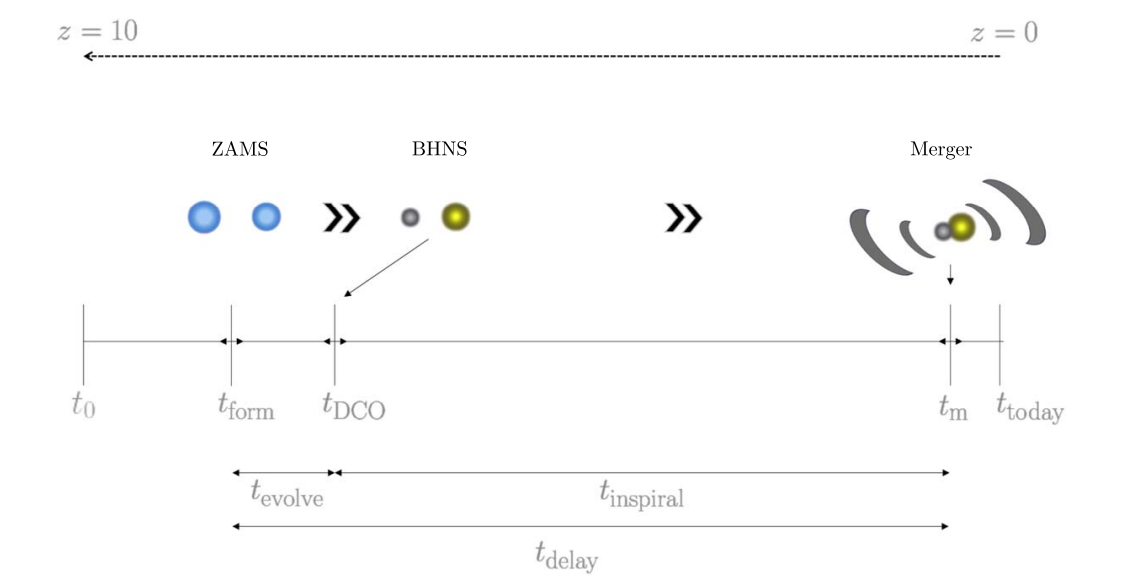
\includegraphics[width=\columnwidth]{images/binary_evolution}%
        \caption{Schematic diagram showing various time intervals for a binary system from ZAMS formation, to DCO, and merger. The figure is taken from~\cite{Riley2022}.}%
        \label{fig:binaryevolution}%
    \end{figure}%

    Once the DCOs have been formed, we move out of the COMPAS suite.
    For the LISA detection, the DCO formed from the set of binaries were checked for an evolutionary stop, i.e., only those binaries were selected that will merge within the Hubble time.
    The selected candidates were than provided to the python framework LEGWORK~\cite{Wagg2021LW} that evolved them from the DCO stage to the merger state.
    It evolved the binaries using equations from~\cite{Peters1963, Peters1964}.

    The DCO$-$merger evolution method follows the one outlined by~\cite{Wagg2021} closely.
    The evolution was done such that the MW galaxy instance was divided into bins based on the metallicity values of the evolving binaries.
    The evolution time was calculated after taking into consideration the ZAMS-DCO evolution time and the lookback time of all the MW points within the metallicity bins.
    If a binary, at DCO stage, had a resultant merger time greater than the difference of its lookback time and ZAMS-DCO evolution time, it was marked as an inspiralling binary.
    Each inspiralling binary was than evolved at every point within the corresponding metallicity bin using LEGWORK to a million year before its merger time.
    At this stage, the resulting LISA parameters of interest were,
    \begin{equation}%
        \semaxis{LISA}, \ecc{LISA}, f_{\text{LISA}}
        \label{eq:lisa_parameter_names}
    \end{equation}%
    The SNR was than calculated by further evolving them for the LISA mission duration of four years.
    The detection is made based on the signal-to-noise ratio (SNR) of the binary averaged over sky position, polarization, and orientation using the following expression from~\cite{Finn2000},
    \begin{equation}
        \rho^2 = \sum_{n=1}^{\infty}\int_{f_{n, i}}^{f_{n, f}}\frac{h_{c, n}^2}{f_n^2 S_n(f_n)}\,\text{d}f_n,
        \label{eq:snr_equation}
    \end{equation}
    where $n$ is the GW harmonic, $f_n$ represents the orbital frequency of $n^\text{th}$ harmonic.
    The parameter $S_n(f_n)$ is the LISA sensitivity curve function~\cite{Robson2019}, and $h_{c, n}$ is the characteristic strain of the $n^\text{th}$ GW harmonic~\cite{Barack2004}.
    \begin{equation}
        h_{c,n}^2 = \frac{2^{5/3}}{3\pi^{4/3}}\frac{(G\mathcal{M}_c)^{5/3}}{c^3 D_L^2}\frac{1}{f_\text{orb}^{1/3}}\frac{g(n, e)}{nF(e)}
        \label{eq:characteristic_strain}
    \end{equation}


    \section{Evolution and detection}
    \label{sec:evolution-and-detection}

    After running the simulations as outlined in section~\ref{sec:population_synthesis}, we obtained 12254 DCOs ($\sim0.12254\%$).
    Following section~\ref{sec:evolution-methodology}, we obtain the required parameter values of only 6539 DCOs that merged within Hubble time ($\sim$53.3621\%) thus making them a potential LISA source.\footnote{Overall, only $\sim$0.06539\% binary system formed into DCOs that merge within Hubble time.}
    The Hubble time merge rate of DCOs is given in table~\ref{tab:dco_details},
    \begin{table}[!ht]%
        \centering
        \resizebox{!}{!}{
            \begin{tabular}{@{}ccccc@{}}
                \toprule
                \multirow{2.5}{*}{Type} & \multirow{2.5}{*}{BHBH} & \multirow{2.5}{*}{NSNS} & \multicolumn{2}{c}{BHNS} \\ \cmidrule(l){4-5}
                &                        &                          & NSBH                   & BHNS                    \\ \midrule
                \notFraction{M}{T} & \notFraction{492}{663} & \notFraction{4752}{9219} & \notFraction{480}{868} & \notFraction{815}{1504} \\
                \notFraction{D}{M} & \notFraction{348}{492} & \notFraction{1281}{4752} & \notFraction{300}{480} & \notFraction{327}{815} \\ \bottomrule
            \end{tabular}%
        }
        \caption{\textsc{\textbf{RowI}} shows the merging (M) vs total (T) formed DCOs in this study, \textsc{\textbf{RowII}} shows the uniquely detectable (D) vs the merging (M) DCOs from this study for $\Theta_1$.}
        \label{tab:dco_details}
    \end{table}

    The highest merging rate in this study is of BHBH pairs ($\sim$74.21\%), followed by NSBH pairs ($\sim$55.30\%), BHNS ($\sim$54.19\%) and lastly NSNS DCO type ($\sim$51.55\%) comprising the `candidate binaries', see table~\ref{tab:dco_details} \textsc{\textbf{RowI}}.\footnote{Such DCO pairs which can have a potential LISA detection.}

    Using the LEGWORK framework~\cite{Wagg2021LW}, these binaries were than checked for their inspiral phase using the $\interval{evolve}$\footnote{Obtained via COMPAS.} and $\interval{lookback}$\footnote{Obtained via galaxy synthesis.}.
    The difference between lookback and evolution time of a binary was required to be less than its merger time\footnote{Obtained via LEGWORK framework.}.
    Out of the merging binaries, BHBH pairs had the most detectable sources in the data set, ($\sim$70.73\%), followed by NSBH pair ($\sim$62.5\%), BHNS pair ($\sim$40.12\%) and lastly NSNS pair ($\sim$26.96\%), see table~\ref{tab:dco_details} \textsc{\textbf{RowII}}.

    As the number of detectable binaries in our study was small compared to the total generated population,\footnote{Due to not using any technique that forces DCO production, e.g., STROOPWAFEL~\cite{Broekgaarden2019}.} multiple detections of a single binary object are present in the final output.
    Table~\ref{tab:bhbh-details-table} shows selective details about mass of progenitor and their evolutionary ends for maximum and minimum mass at ZAMS and DCO stages.
    In appendix~\ref{sec:paramter-distribution-across-the-galaxies} we present the number of detection and mean values for selected parameters\footnote{The selected parameters include, $\mone{DCO}$, $\mtwo{DCO}$, $\semaxis{DCO}$, $\ecc{DCO}$, Z, $\interval{evol}$, $\interval{lookback}$, and SNR.} across the hundred instances of MW galaxies.
    The number of detections across all the MW instances came out to be 12841.

    \begin{table}[!h]
        \centering
        \resizebox{\columnwidth}{!}{%
            \begin{tabular}{@{}ccccccccccc@{}}
                \toprule
                \multirow{2.5}{*}{Parameters} & \multirow{2.5}{*}{MAX} & \multicolumn{2}{c}{ZAMS details} & \multicolumn{2}{c}{DCO details} & \multirow{2.5}{*}{MIN} & \multicolumn{2}{c}{ZAMS details} & \multicolumn{2}{c}{DCO details} \\ \cmidrule(lr){3-4} \cmidrule(lr){5-6} \cmidrule(lr){8-9} \cmidrule(lr){10-11}
                &         & Primary & Secondary & Primary & Secondary &        & Primary & Secondary & Primary & Secondary \\ \midrule

                \multicolumn{11}{c}{\textbf{Binary Black Holes}} \\
                $\mone{ZAMS}$ & 149.836 & 149.836 & 115.624   & 10.386  & 10.395    & 13.007 & 13.007  & 12.500    & 2.216   & 2.601     \\
                $\mtwo{ZAMS}$ & 131.178 & 148.802 & 131.178   & 8.662   & 8.459     & 12.500 & 13.007  & 12.500    & 2.216   & 2.601     \\
                $\mone{DCO}$  & 43.308  & 57.334  & 57.334    & 43.308  & 43.308    & 2.022  & 26.497  & 26.493    & 2.022   & 7.104     \\
                $\mtwo{DCO}$  & 43.308  & 57.334  & 57.334    & 43.308  & 43.308    & 2.018  & 42.088  & 30.574    & 7.456   & 2.018     \\

                \multicolumn{11}{c}{\textbf{Binary Neutron Stars}} \\

                $\mone{ZAMS}$ & 54.41   & 54.41   & 13.76     & 1.614   & 1.235     & 8.546  & 8.546   & 7.822     & 1.26    & 1.193     \\
                $\mtwo{ZAMS}$ & 25.571  & 25.586  & 25.571    & 1.480   & 1.693     & 6.626  & 13.01   & 6.626     & 1.26    & 1.194     \\
                $\mone{DCO}$  & 1.938   & 14.022  & 13.938    & 1.938   & 1.487     & 1.135  & 10.319  & 10.019    & 1.135   & 1.392     \\
                $\mtwo{DCO}$  & 1.991   & 13.919  & 13.574    & 1.681   & 1.991     & 1.132  & 11.674  & 11.021    & 1.518   & 1.132     \\

                \multicolumn{11}{c}{\textbf{Neutron Star $-$ Black Hole}} \\

                $\mone{ZAMS}$ & 53.708  & 53.708  & 29.613    & 1.439   & 15.342    & 8.971  & 8.971   & 8.847     & 1.260   & 3.869     \\
                $\mtwo{ZAMS}$ & 42.242  & 42.289  & 42.242    & 1.598   & 7.382     & 8.665  & 9.164   & 8.665     & 1.260   & 2.062     \\
                $\mone{DCO}$  & 1.935   & 14.090  & 13.959    & 1.935   & 3.825     & 1.137  & 27.186  & 17.676    & 1.137   & 9.646     \\
                $\mtwo{DCO}$  & 15.342  & 53.708  & 29.613    & 1.439   & 15.342    & 2.003  & 12.472  & 12.033    & 1.608   & 2.003     \\

                \multicolumn{11}{c}{\textbf{Black Hole $-$ Neutron Star}} \\

                $\mone{ZAMS}$ & 145.467 & 145.467 & 46.439    & 9.907   & 1.593     & 11.626 & 11.626  & 11.608    & 2.216   & 1.522     \\
                $\mtwo{ZAMS}$ & 108.489 & 140.091 & 108.489   & 12.217  & 1.415     & 10.072 & 23.144  & 10.072    & 2.922   & 1.206     \\
                $\mone{DCO}$  & 15.106  & 90.844  & 76.11     & 15.106  & 1.669     & 2.004  & 13.125  & 12.872    & 2.004   & 1.785     \\
                $\mtwo{DCO}$  & 1.945   & 29.142  & 15.445    & 4.341   & 1.945     & 1.141  & 28.317  & 22.834    & 5.61    & 1.141     \\ \bottomrule
            \end{tabular}%
        }
        \caption{Maximum and minimum values for masses of both ZAMS and DCO type stars in the BHBH data set with their respective counterparts. The `MAX' and `MIN' columns represent the maximum and minimum value for the given parameter respectively. The `ZAMS details' and `DCO details' column list the value of primary and secondary components of the binary and respective stage of evolution with `MAX' and `MIN' value of the parameter at that stage. All the masses are given in units of solar mass.}
        \label{tab:bhbh-details-table}
    \end{table}

    The predicted distribution of the LISA detectable sources are plotted over its expected sensitivity curve~\cite{Robson2019}, in figure~\ref{fig:alldcosnrplotting}.
    The x-axis shows the dominant frequency, the frequency accumulating the largest SNR, for the eccentric binaries.
    Furthermore, on y-axis we plot the amplitude spectral density (ASD), including the contribution from all harmonics.
    The gap between the detected binaries and the LISA curve in the graph is the SNR criteria, ($\text{SNR}>7$).
    The size of the points varies with metallicity; high metallic sources have larger shapes and vice versa.
    The color scheme is based on the eccentricity of detected binaries with a reverse red-yellow-green color palette\footnote{\url{https://matplotlib.org/stable/gallery/color/colormap_reference.html}}, going from green, yellow and finally red in increasing order of eccentricity values.

    \begin{figure}[!h]%
        \centering
        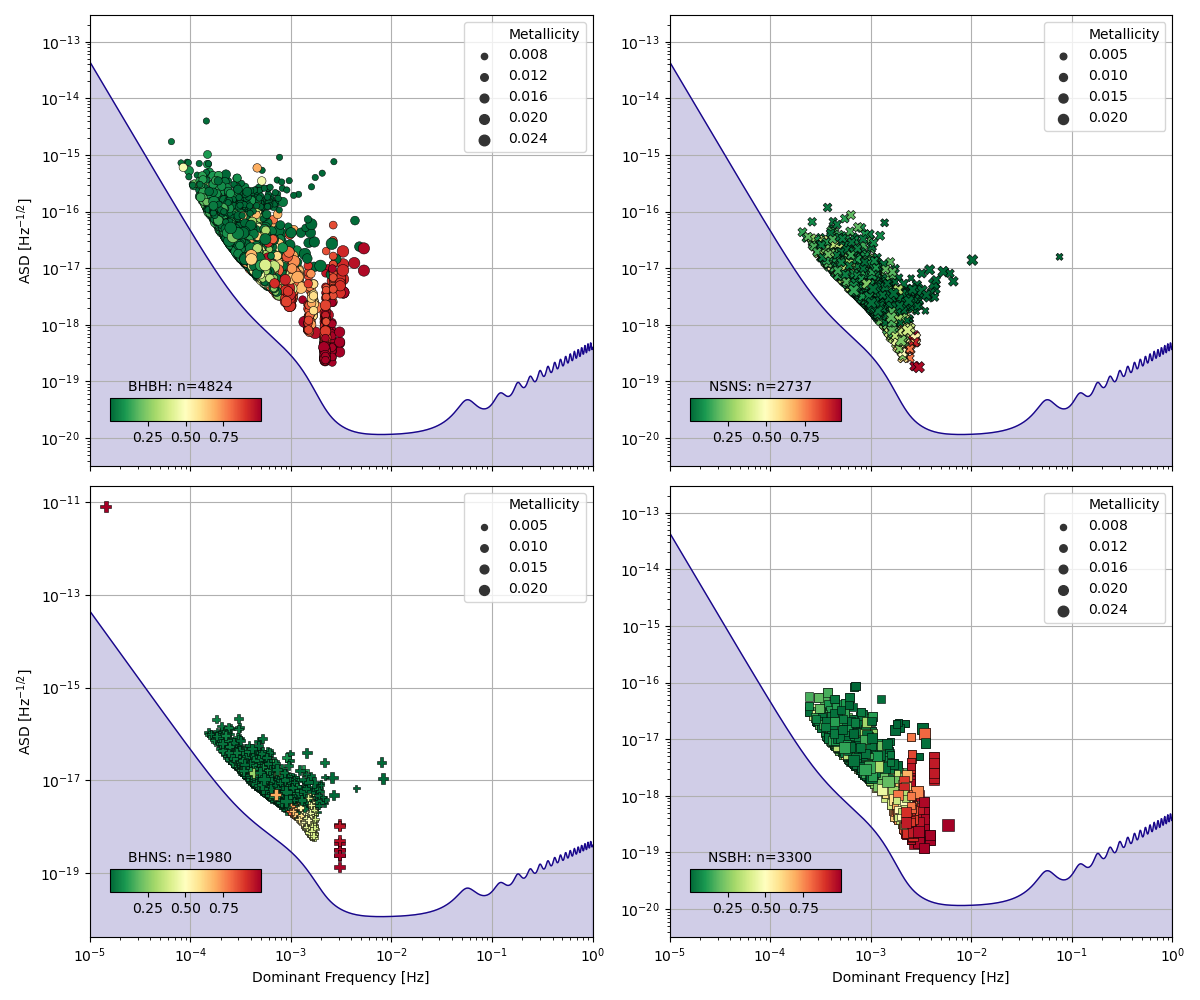
\includegraphics[width=\columnwidth]{analysis_data/004__images_for_latex/dco_typewise_snr}
        \caption{Detectable sources' characteristic strain vs. dominant frequency in our simulations are shown on the LISA sensitivity curve for $\Theta_1$ data set. The sources are color-coded based on their eccentricities, green for low and red for high eccentric sources.}
        \label{fig:alldcosnrplotting}
    \end{figure}

    \begin{figure}[!h]%
        \centering
        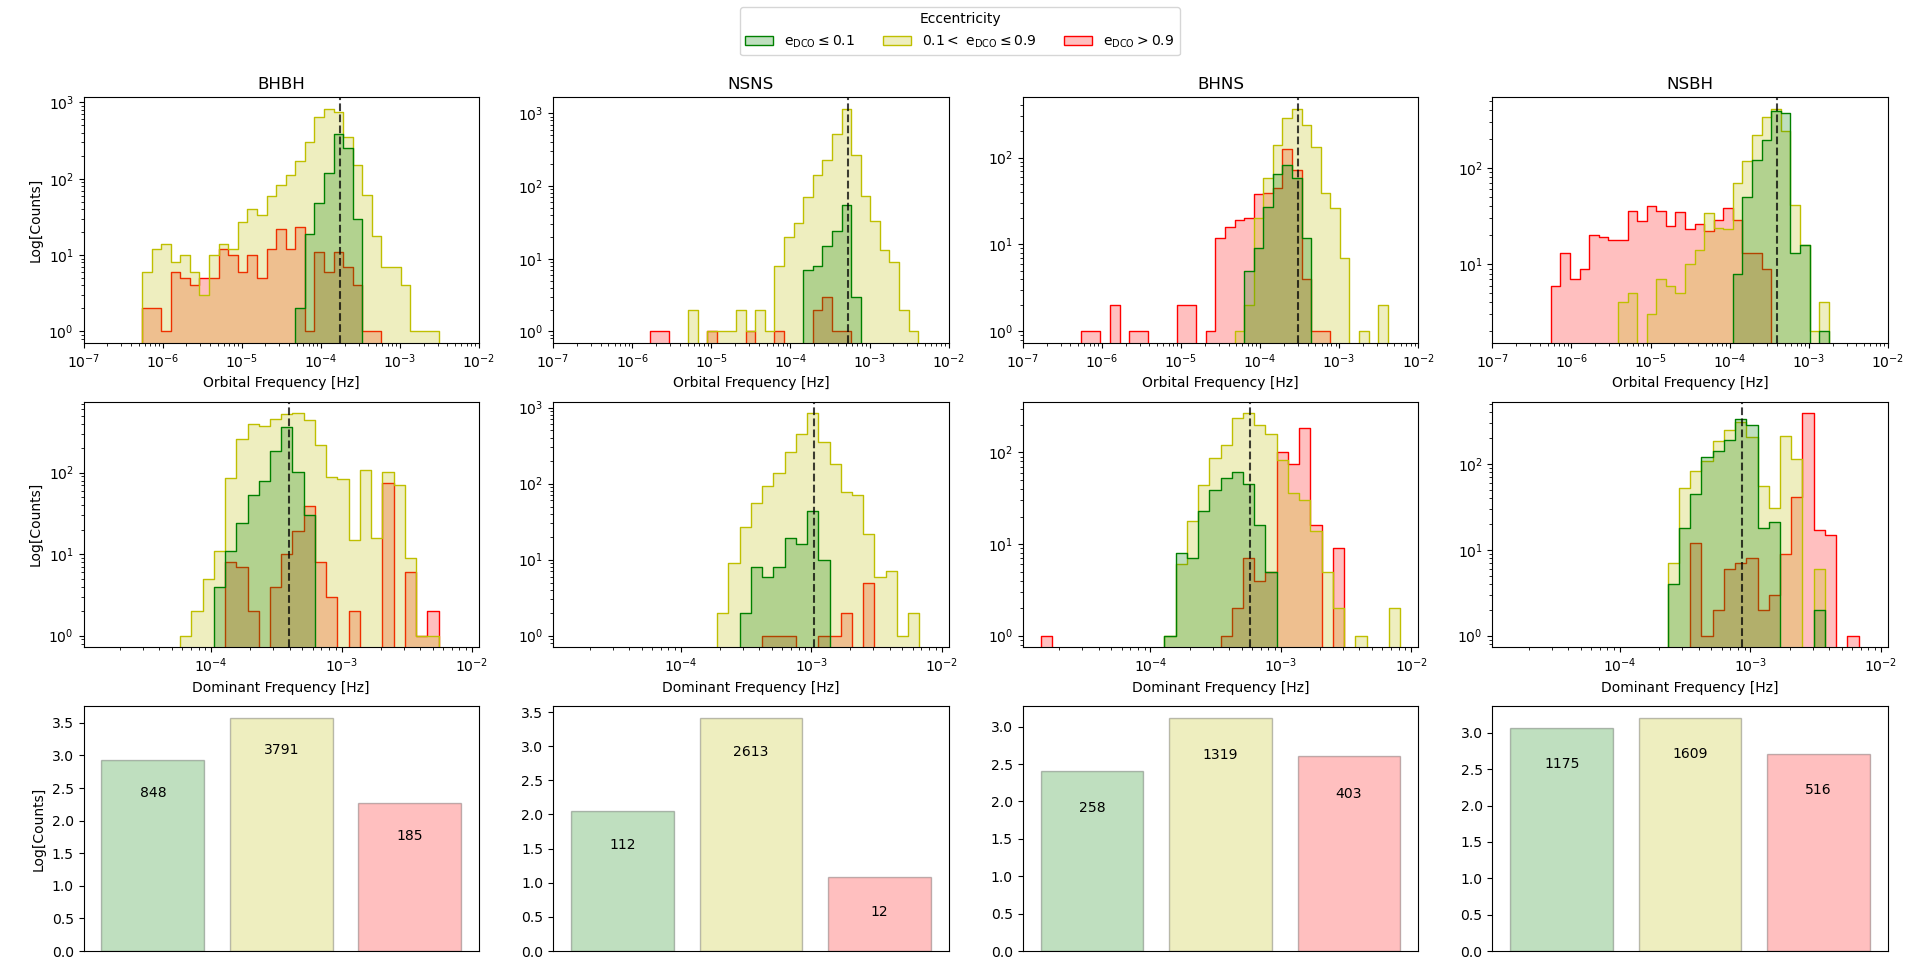
\includegraphics[width=0.9\columnwidth]{analysis_data/004__images_for_latex/dco_fdom_ecc_details}
        \caption{\textsc{\textbf{Row1:}} Eccentricity characterized distribution of DCOs for their orbital frequency. \textsc{\textbf{Row2:}} Same as \textsc{\textbf{Row1}} but for the binary's dominant frequency. \textsc{\textbf{Row3:}} Number of binaries associated with the given eccentricity in log scale. The number inside the bars show the actual number of binaries for the given eccentricity. The log scaling was chosen due to relative lower number of DCOs in NSNS and BHNS types.}
        \label{fig:dcofdomeccdetails}
    \end{figure}%

    Majority of the binary population reside on the lower end of LISA spectrum.
    For \textsc{\textbf{Row1}}, the peak orbital frequency occurs at \SI{0.174}{\milli\hertz}, \SI{0.5308}{\milli\hertz}, \SI{0.3039}{\milli\hertz}, and \SI{0.4016}{\milli\hertz} respectively for BHBH, NSNS, BHNS and NSBH population.
    Similarly, for \textsc{\textbf{Row2}}, the peak dominant frequency occurs at \SI{0.3919}{\milli\hertz}, \SI{1.057}{\milli\hertz}, \SI{0.5828}{\milli\hertz}, and \SI{0.8668}{\milli\hertz} respectively.
    The reason for such a trend can be explained through the eccentricities of the binaries.
    As seen from the figure~\ref{fig:dcofdomeccdetails} \textsc{\textbf{Row3}}, a large portion of our binaries is either low or mid-eccentric.
    The orbit of low eccentric binaries evolves differently than high eccentric binaries.
    After the formation of DCO, the low eccentric binaries emit GW in the second harmonic of their orbital frequency.
    The intensity of the frequency increases as the orbits starts to shrink.
    On the other hand, the DCOs with high eccentricities behave in a completely different way, i.e.\ their orbit decay faster, and they tend to emit GW in high harmonics~\cite{Peters1963, Peters1964}.
    This also explains why even though the orbital frequency of the high eccentric binaries was small but they have larger dominant frequency.

    We also notice a stray binary pair in BHNS with an ASD $\sim$\SI{8e-12}{\hertz\tothe{1/2}}, the highest in $\Theta_1$.
    The parameter of that particular BHNS pair are presented in table~\ref{tab:bhnsbinarydetails}.
    It is important to note that before the binary's evolution for SNR detection, it had originally evolved past its look-back time.
    With a lookback time of $\sim$\scientific{10.393}{\mega\yr} and evolution time of $\sim$\scientific{10.944}{\mega\yr}, the merging time for this binary came out to be only $\sim$\scientific{3.83}{\yr} when put into LEGWORK\@.
    This also explains why the parameters of this binary are identical when considering the DCO stage and near merging stage after evolving via LEGWORK\@.
    The system is emitting a dominant frequency of $\sim$\SI{1.439e-5}{\hertz} at a harmonic of 1, which makes it exactly the same as its orbital frequency.

    \begin{table}[!h]%
        \centering
        \resizebox{\columnwidth}{!}{%
            \begin{tabular}{@{}ccccccc@{}}
                \toprule
                \wraptablerow{Binary}{Stage} & \wraptablerow{$m_1$}{$[\si{\Msun}]$} & \wraptablerow{$m_2$}{$[\si{\Msun}]$} & \wraptablerow{$a$}{\si{\AU}} & $e$ & $Z$ & $\o$\\ \midrule
                ZAMS                         & 33.449                               & 17.711                               & 0.666                        & 0.153 & 0.024 & 8848207 \\
                \notFraction[\&]{DCO}{LISA}  & 6.495                                & 1.407                                & 0.034                        & 0.999 & //    & //      \\  \bottomrule
            \end{tabular}%
        }
        \caption{Parameters at difference stages of binary evolution for BHNS pair with seed number 8848207.}
        \label{tab:bhnsbinarydetails}
    \end{table}%

    \begin{figure}[!h]%
        \centering
        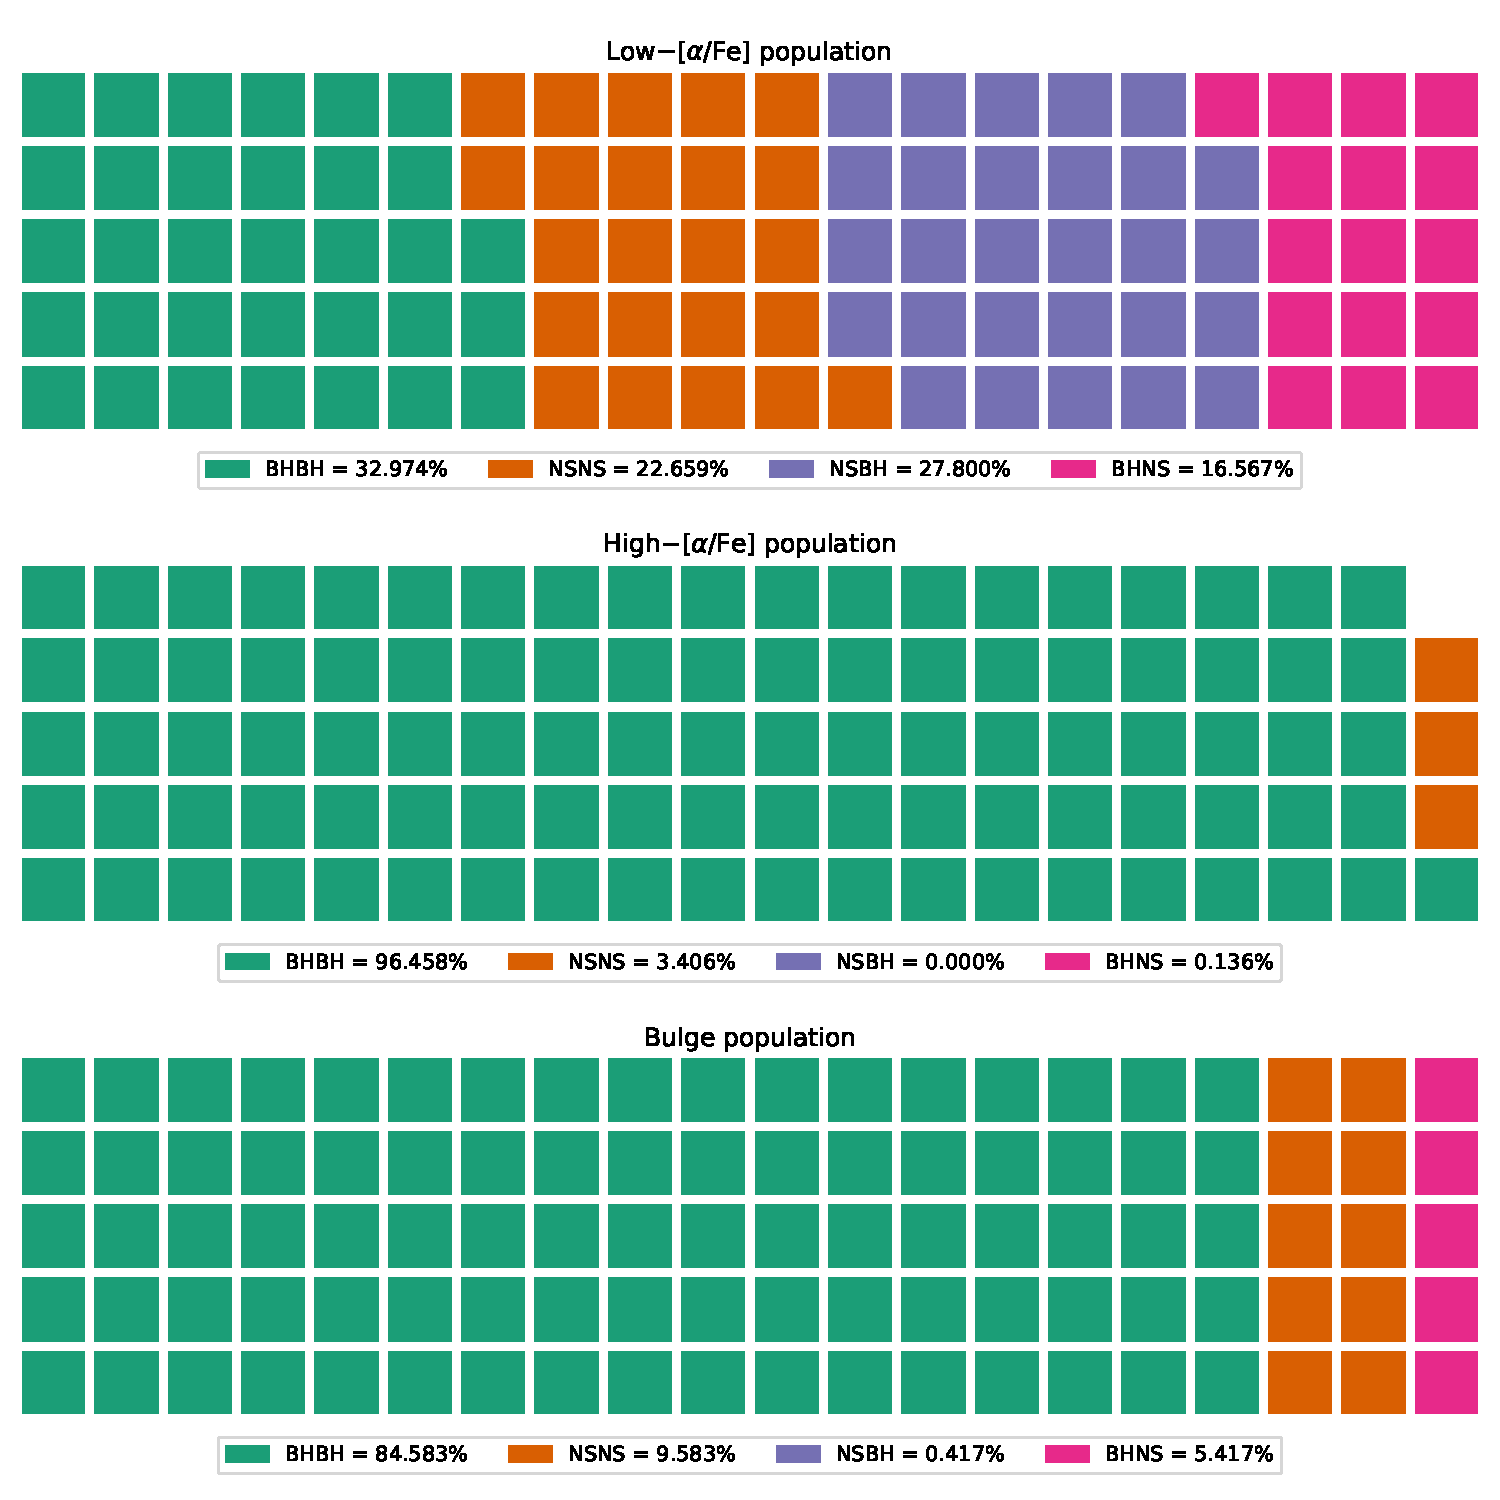
\includegraphics[width=\columnwidth]{analysis_data/004__images_for_latex/dco_type_MW_component_distribution}
        \caption{Waffle charts showing percentage proportion for DCO type detections in the MW instance components in this study.}
        \label{fig:dcotypemwcomponentdistributioncropped}
    \end{figure}%

    Figure~\ref{fig:dcotypemwcomponentdistributioncropped} shows the percentage of different DCOs detected in the \lowalpha, \highalpha and bulge components of the MW instances.
    For \lowalpha\ disk, the NSBH pairs have more detections than BHN pairs.
    Contrary to that, NSBH pairs show no detection in \highalpha\ disk, and fractional detection in the bulge, $\sim0.833\%$.
    On the other hand, the BHNS pairs have the lowest detection rate in all three components.

    BHBH is the dominant detectable pair in all three components.
    Except for the \lowalpha\ component, the NSNS pair also has higher percentage of detection.
    For the \lowalpha\ component we see a higher percentage of NSBH detection.
    \begin{figure}[!h]%
        \centering
        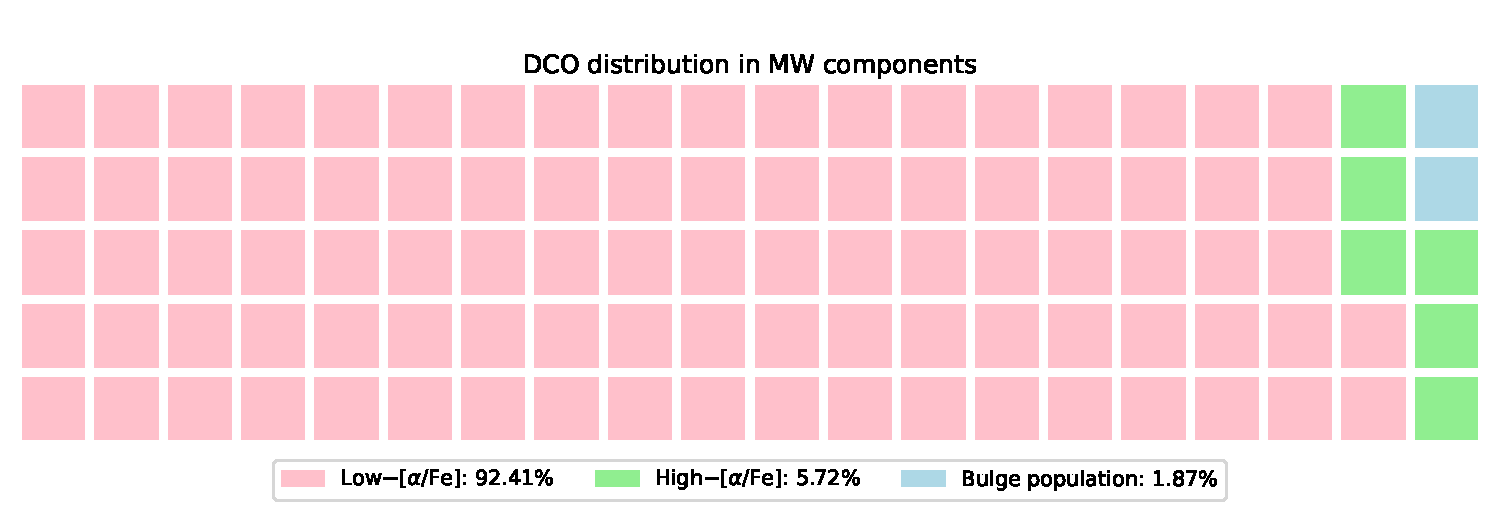
\includegraphics[width=\columnwidth]{analysis_data/004__images_for_latex/dco_type_MW_distribution}
        \caption{Waffle chart showing the total number of detections per MW instance component in this study on the whole.}
        \label{fig:dcotypemwdistribution}
    \end{figure}%

    Figure~\ref{fig:dcotypemwdistribution} shows the percentage of detections in the three components regardless of the DCO type.
    Here we see that majority of the detections are in the \lowalpha\ disk.
    This can be attributed to the biased metallicity value used in this study, $\text{Beta}(5, 80)$.
    These detection percentages do align with the age-metallicity relationship as the bulge is oldest component and thus should have lower metallicity ZAMS stars.
    However, due to the choice of metallicity distribution, these stars were not generated in large numbers.

    \subsection{Maximum distance}\label{subsec:maximum-distance}
    For each DCO, there is a horizon distance i.e., the maximum distance up to which the DCO may be detect\@.ble in LISA\@.
    This is calculated using the inverse relationship between SNR ($\rho$) and distance~\cite{Lau2020},
    \begin{equation}
        \label{eq:eq1}
        d_\text{max}=\frac{\rho(d=1\,\text{kpc})}{\rho_\text{min}}
    \end{equation}

    Where $\rho_{\min}$ is the minimum value of SNR below which the source is not detectable.
    We keep the detection threshold at $\rho_{\min}=7$, and $\rho(d=1\,\text{kpc})$ is SNR of the source if it was at $1\,\text{kpc}$ distance from the detector.
    We calculated the SNR of all the detected sources at \SI{1}{\kpc} distance using the python package LEGWORK~\cite{Wagg2021LW}.
    Afterward, their maximum distances $(d_{\max})$ were calculated.

    Figure~\ref{fig:dmax} shows the mean maximum distances for all the detected sources.
    The black line shows the average maximum distance for all the types combined.
    The LISA sensitivity curve is also overlaid on the graph.

    \begin{figure}[!h]
        \centering
        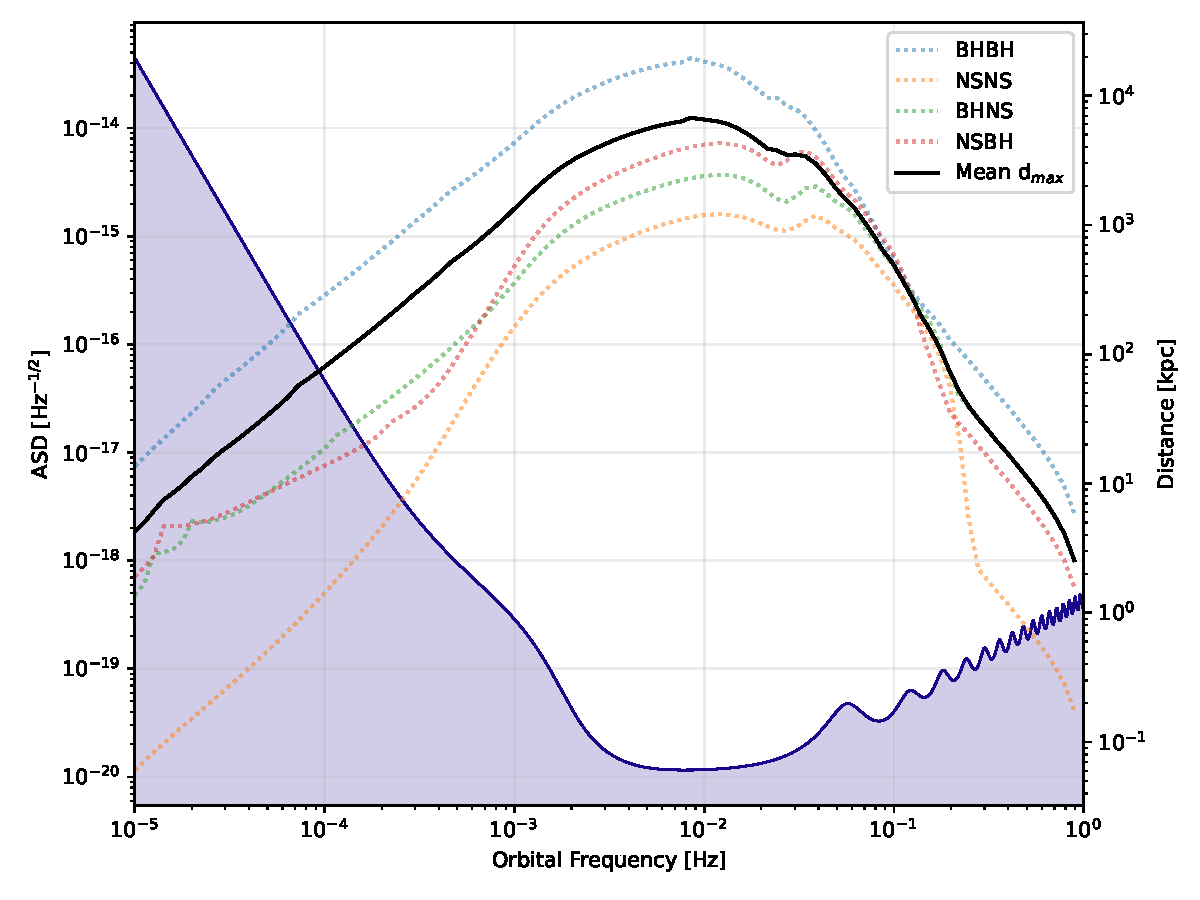
\includegraphics[width=\linewidth]{analysis_data/004__images_for_latex/d_max}
        \caption{Mean maximum distances for all of the different types of DCO corresponding to their orbital frequency. The overall average maximum detection distance is shown by a black line.}
        \label{fig:dmax}
    \end{figure}

    BHBH pairs can be observed up to an average distance of $\sim$\scientific{1.95e4}{\kpc}.
    For NSNS, BHNS, and NSBH the maximum distance came out to be $\sim$\scientific{1.21e3}{\kpc}, $\sim$\scientific{4.28e3}{\kpc}, and $\sim$\scientific{2.43e3}{\kpc} respectively.
    The combined mean maximum distance comes out to be $\sim$\scientific{6.74e3}{\kpc}.

    We also observe that the maximum distance for all the binaries is observed around the dominant frequency right around the LISA's most sensitive region, e.g., \scientific{10}{\milli\hertz}.
    For BHBH, the maximum distance is observed at \scientific{8.498e-3}{\hertz}.
    The NSNS, BHNS, and NSBH pairs show the maximum distance value at the same frequency, \scientific{1.205E-02}{\hertz}.
    However, when taking the mean for all four DCO types, the dominant frequency corresponding to the maximum distance changes back to \scientific{8.498E-3}{\hertz} showing the effects of the most dominantly detected DCO type, BHBH\@.


    \section{Comparative analysis}
    \label{sec:comparative-analysis}
    In this section, we will deal with the comparative study of our two data sets, $\Theta_1$ and $\Theta_2$.
    In order to fairly compare the two, given only the difference of eccentricity, we make use of the seed numbers provided in $\Theta_1$ data set.
    With the exception of SN kick parameters and eccentricity, all the other parameters were kept the same as in the original data set.
    We evolved the binaries for $\Theta_2$ consistent with the method described in this paper.
%    We first briefly discuss the output parameters for $\Theta_2$,

    \subsection{Hubble Merger Rate}
    \label{subsec:hubblemergerrate}
    After running the simulations, we obtained 9751 DCO pairs ($\sim0.09751\%$). Out of these, only 5178 ($\sim53.1022\%$) were able to merge within Hubble time, (see table~\ref{tab:dco_details0e}).

    From table~\ref{tab:dco_details0e} \textsc{\textbf{RowI}} we observe that the highest merging rate comes from BHBH as well ($\sim$66.32\%), followed by BHNS pairs ($\sim$65.87\%), NSBH ($\sim$63.03\%) and lastly, NSNS dco type ($\sim$51.57\%).

    Table~\ref{tab:dco_details0e} \textsc{\textbf{RowII}} shows that we have NSBH as the dominant detectable DCO type ($\sim$77.93\%) detections instead of BHBH as in $\Theta_1$ data set.
    This is followed by BHBH pairs ($\sim$77.25\%), BHNS pairs ($\sim$68.91\%) and lastly, NSNS pairs ($\sim$17.46\%).

    \begin{table}[!ht]%
        \centering
        \resizebox{!}{!}{
            \begin{tabular}{@{}ccccc@{}}
                \toprule
                \multirow{2.5}{*}{Type} & \multirow{2.5}{*}{BHBH} & \multirow{2.5}{*}{NSNS} & \multicolumn{2}{c}{BHNS} \\ \cmidrule(l){4-5}
                &                        &                          & NSBH                   & BHNS                   \\ \midrule
                \notFraction{M}{T} & \notFraction{189}{285} & \notFraction{4438}{8605} & \notFraction{358}{568} & \notFraction{193}{293}  \\
                \notFraction{D}{M} & \notFraction{146}{189} & \notFraction{775}{4438}  & \notFraction{279}{358} & \notFraction{133}{193} \\ \bottomrule
            \end{tabular}%
        }
        \caption{\textsc{\textbf{RowI}} shows the merging (M) vs total (T) formed DCOs in this study, \textsc{\textbf{RowII}} shows the uniquely detectable (D) vs the merging (M) DCOs from this study for $\Theta_2$.}
        \label{tab:dco_details0e}
    \end{table}

    The only particular DCO type with a noticeable effect of ZAMS eccentricity is the NSNS type which shows a lot of detections given that the binaries start with eccentric orbits.

    \subsection{Detection rates}
    \label{subsec:detectionetection-rates}
    The $\Theta_2$ data set shows an overall slight increase in the detection rate, $(86-131)$ detections against $(83-124)$ detection for $\Theta_1$ data set.
    Although minor overall, the detection rate is significant for BHNS, and NSBH pairs going from $(6-28)$ and $(13-39)$ in $\Theta_1$ to $(11-29)$ and $(21-46)$ respectively for $\Theta_2$ over a four year LISA mission.

    Similar to appendix~\ref{sec:paramter-distribution-across-the-galaxies} for $\Theta_1$, appendix~\ref{sec:paramter-distribution-across-the-galaxies-theta-2} shows the distribution of parameters and average number of DCO detections across the ensemble of the galaxies in this study for $\Theta_2$.
    The difference in average number of BHNS detections in the two data set is $\sim$18, the largest, jumping from 33 to 51 for $\Theta_1$ and $\Theta_2$ respectively.
    Similarly, the NSBH binaries show an average increase of 3 detections.
    As for BHBH and NSNS pairs, there are more detections in $\Theta_1$ compared to $\Theta_2$.

    It is also noted that the mean parameter values for $\Theta_2$ are also higher than $\Theta_1$ for BHNS, and NSBH pairs, but this might be because of the increased number of detections and vice versa for BHBH, and NSNS pairs.

    \subsection{Maximum detection distance}
    \label{subsec:maximumdetectiondistance}
    Figure~\ref{fig:dmaxdifference} shows the ratio of maximum detection distance between $\Theta_2$ and $\Theta_1$.
    We note that the ratio is less than 1 at lower orbital frequencies, from \SIrange{1e-5}{1.15e-4}{\hertz} after which is increases and only comes below 1 around \SIrange{1.232e-1}{1.384e-1}{\hertz}.
    This suggests that the binaries with circular ZAMS orbits will evolve such that they can be detected to larger distances compared to one with eccentric ZAMS orbits in LISA sensitive band.

    \begin{figure}[!h]
        \centering
        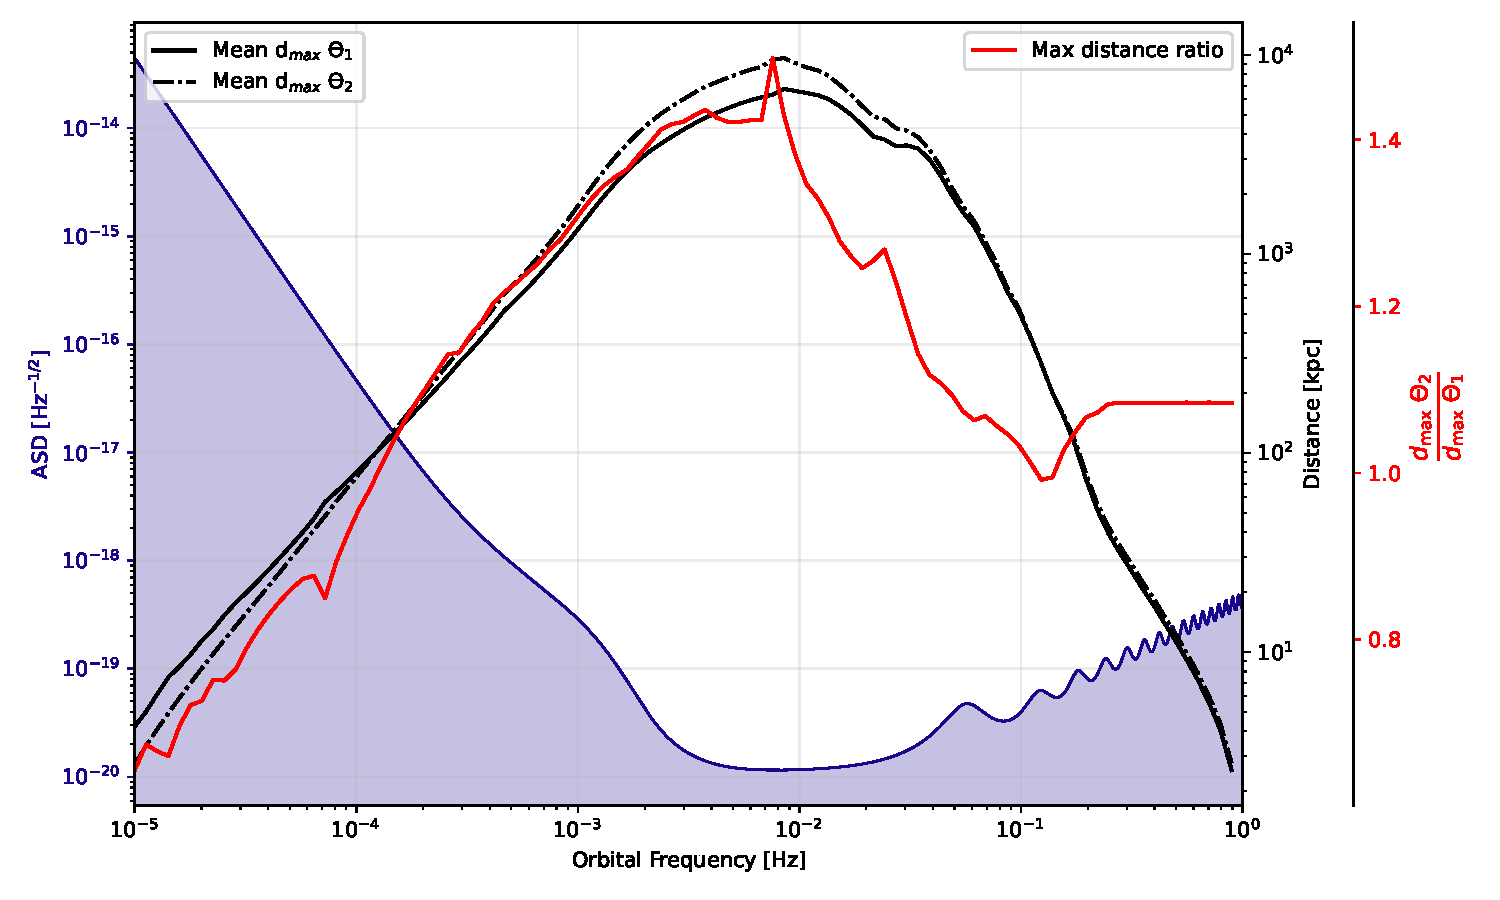
\includegraphics[width=\columnwidth]{analysis_data/004__images_for_latex/d_max_difference}
        \caption{Mean maximum distance of the two data sets, black solid and dashed lines, and their ratio, red solid line.}
        \label{fig:dmaxdifference}
    \end{figure}

    \subsection{Two interesting NSNS binaries}
    \label{subsec:twointerestingnsnsbinaries}

    Appendix~\ref{sec:paramter-distribution-across-the-galaxies-theta-2} figure~\ref{fig:nsbh0endetections} shows a spike in the NSNS SNR plot.
    This is due to an extremely high value of SNR found in the simulated galaxy number 43, with an average $\log_{10}$(SNR) of $1.6864\pm2.7482$.
    The maximum SNR in that galaxy is of the binary at seed number 6308709.
    The particulars of this binary are given in table~\ref{tab:weirdnsns}.
    The values in the table are rounded off for display purposes.

    \begin{table}[!hb]%
        \centering
        \resizebox{!}{!}{
            \begin{tabular}{@{}cccc@{}}
                \toprule
                $\mone{DCO}$     & $\mtwo{DCO}$                      & $m_\text{chirp}$      & $\semaxis{DCO}$      \\
                1.26\,\si{\Msun} & 1.91\,\si{\Msun}                  & 1.35\,\si{\Msun}      & 0.044\,\si{\AU}      \\ \midrule[1pt]
                $\ecc{DCO}$      & Z                                 & $t_\text{evol}$       & $t_\text{lookback}$  \\
                0.9999           & 0.02595                           & 30.135\,\si{\mega\yr} & 4.967\,\si{\mega\yr} \\ \midrule[1pt]
                SNR              & \wraptablerow{MAX SNR}{harmonics} & Galaxy                & \o                   \\
                \num{6.8467e14}  & 2                                 & 43                    & 6308709              \\ \bottomrule
            \end{tabular}
        }
        \caption{Parameters of the NSNS pair with highest SNR in galaxy number 43.}
        \label{tab:weirdnsns}
    \end{table}%

    \begin{figure}[!h]%
        \centering
        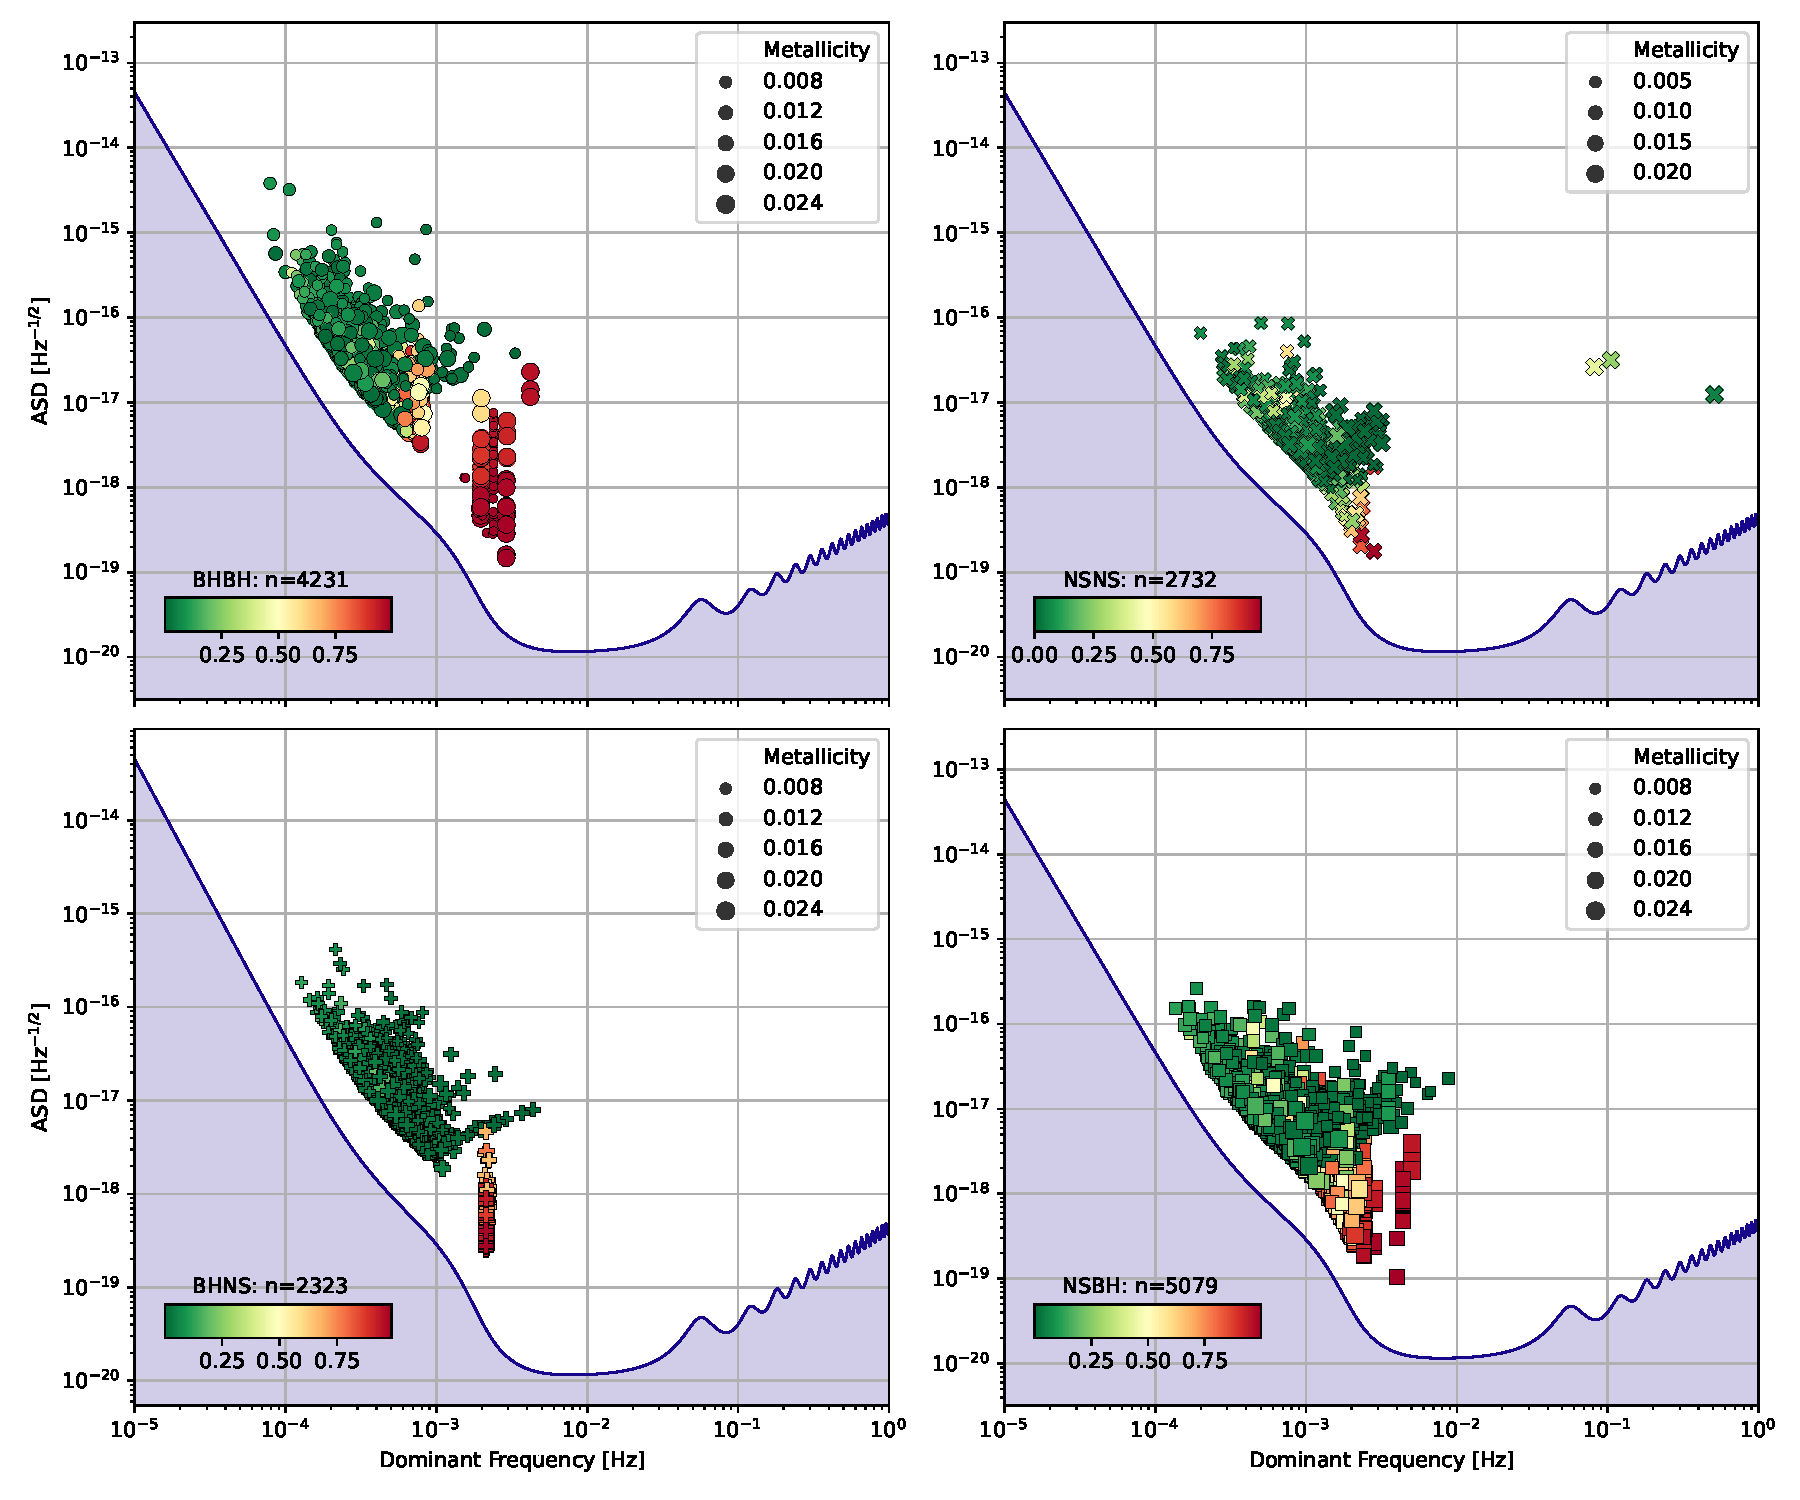
\includegraphics[width=\columnwidth]{analysis_data/004__images_for_latex/dco_typewise_snr0e}
        \caption{Same as figure~\ref{fig:alldcosnrplotting} but for $\Theta_2$ data set.}
        \label{fig:dcotypewisesnr0e}
    \end{figure}%

    Upon further investigations, we came to know that the binary might have merged already.
    The LISA parameters, $\ecc{LISA}, \semaxis{LISA}, f_\text{LISA}$, for said binary show that the semi-major axis and eccentricity for this binary at the time of SNR detection are \num[scientific-notation=engineering]{8.66e-51}\,AU and \num[scientific-notation=engineering]{1.034e-71} respectively.
    The extremely high SNR also accompanies an equally high dominant frequency, out of the plotting range, of roughly \num{1.4e68}\,\si{\hertz} and an undefined ASD value.
    We show the detections of $\Theta_2$ is figure~\ref{fig:dcotypewisesnr0e}.
    The binary discussed above, with seed number 6308709, is not visible in this plot.

    There are three more NSNS detections that are out of characteristics, and all three are the same pair with seed number 1699345.

    \begin{table}[!h]
        \centering
        \resizebox{!}{!}{
            \begin{tabular}[c]{@{}ccccc@{}}
                \toprule
                \multicolumn{5}{c}{LISA parameters for $\o = 1699345$} \\\midrule
                & \wraptablerow{$f_\text{orb}\times10^{-3}$}{$\si{\hertz}$} & \wraptablerow{$f_\text{dom}\times10^{-17}$}{$\text{Hz}^{-1/2}$} & \wraptablerow{$\semaxis{LISA}\times10^{-3}$}{$\si{\Rsun}$} & $\ecc{LISA}$\\\midrule
                1 & \num{27.318}                                              & \num{2.611}                                                     & \num{35.384}                                               & \num{0.4175} \\
                2 & \num{52.504}                                              & \num{3.155}                                                     & \num{22.890}                                               & \num{0.2601} \\
                3 & \num{255.01}                                              & \num{1.236}                                                     & \num{7.981}                                                & \num{0.0554} \\\bottomrule
            \end{tabular}
        }
        \caption{LISA parameters for binary with $\o = 1699345$ obtained by LEGWORK before SNR calculations.}
        \label{tab:parameters1699345}
    \end{table}

    \subsection{Final evolutionary stages}
    \label{subsec:finalevolutionarystages}
    A total of 137 seeds were found common between the two data sets.
    Out of these 137 seeds, 104 were found to evolve to the same final stage in both data sets.
    The binaries with common and diverging final evolutionary stages are shown in figure~\ref{fig:dcotypedivergenceintwodatasets}.
    The lesser number of diverging cases indicate that the ZAMS eccentricity might not play as much of a bigger role in the development of binary's final stages.

    For a better understanding of what the plot is showing, consider the two points highlighted.
    The red marker on the tail of the arrow shows the DCO stage for the binary in $\Theta_1$ data set, the arrow indicates direction of divergence in evolution with the arrow head showing the final DCO stage of the same binary in $\Theta_2$ data set.
    On the other hand, the cyan marker indicates no divergence in the evolution, meaning that the binary had the same final evolution stage in both the data sets.
    The particular binaries in question have seed numbers, 44735 and 1367057 respectively.

    \begin{sidewaystable}
        \centering
        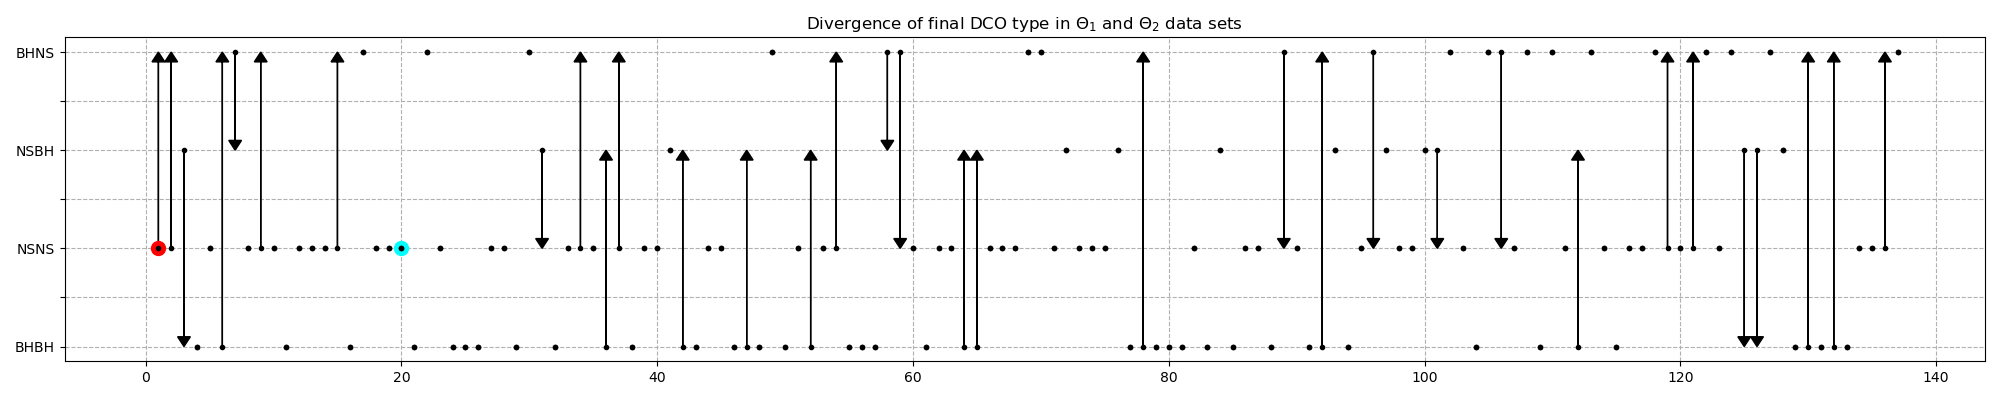
\includegraphics[width=\textwidth]{analysis_data/004__images_for_latex/dco_type_divergence_in_two_datasets}
        \captionof{figure}{Plot showing the change in DCO ending states for the common seed numbers from $\Theta_1$ and $\Theta_2$ data sets. The direction of arrows shows the change in the DCO type from $\Theta_1$ and $\Theta_2$ data set. The binaries that didn't change the DCO type after evolution are represented by a filled dot.}
        \label{fig:dcotypedivergenceintwodatasets}
    \end{sidewaystable}


    \section{Conclusion}
    \label{sec:conclusion}

    We simulated \num{1e7} binaries using COMPAS suite, evolving them to their DCO stage with non-zero ZAMS metallicity.
    We only chose those DCOs that were able to merge within the Hubble time as our working data set.

    In a separate phase, we made use of the metallicity-dependent model to create one hundred instances of MW galaxy mimicking near present metallicity conditions.
    Each instance was partitioned into metallicity bins depending upon the number of DCOs that merged within the Hubble time.
    The bins were selected such that the metallicity closest to the binary was kept in the center of the bin.
    The binaries were than evolved at each point in the bin keeping in view the different distances associated with the points generated in the MW galaxy through LEGWORK\@.
    This evolution was performed for same binaries in all galaxy instances sequentially, generating a large data set of multiple distance-based detections of the binaries.

    When averaged over a hundred random MW instances, we detected 50, 27, 20, and 33 detections for BHBH, NSNS, BHNS, and NSBH pairs respectively.
    Due to the underlying metallicity distribution, majority of the binaries were detected in the \lowalpha\ component of the galaxy.
    We observe a relatively large number of BHNS pairs in contrast to NSBH pairs in the output.
    Using the maximum detection distance formula, we observe the dco pairs to be, on average, detectable up to \SI{5}{\mega\parsec}.

    When compared to a similar data set but with circular ZAMS eccentricities, we see a similar percentage detection but fewer number of detections for each DCO type.
    However, the NSBH pairs show a huge increase in detection, going from 33 detections to 51.
    Majority of the common detected binaries in both the data sets converged to the same DCO stage, which might indicate that the initial eccentricity parameter is not so significant in determining the final DCO stages.
    It is also interesting to note that majority of the converging binaries\footnote{Fifteen.} tend to go towards BHNS pair.
    On the other hand, only three, five and six binaries converged towards BHBH, NSBH, and NSNS DCO stage respectively.

    \cleardoublepage
    \bibliographystyle{others/apj}
    \bibliography{reference}
    \cleardoublepage
    \appendices
    \section{Settings for using COMPAS}
\label{sec:appA}
To generate a binary system in COMPAS, we require the following parameters as discussed earlier,
\begin{itemize}
    \item mass of primary star $(\mone{ZAMS})$,
    \item mass of secondary star $(\mtwo{ZAMS})$,
    \item semi-major axis of the orbit $(\semaxis{ZAMS})$,
    \item random seed $(\o)$
    \item remnant mass prescription,
    \item eccentricity of the orbit $(\ecc{ZAMS})$, and
    \item metallicity of the stars $\left(Z\right)$.
\end{itemize}

We've discussed the first four parameters in the main text, here we will discuss the selection of eccentricity and metallicity values.

\subsection{\textbf{Eccentricity}}
\label{subsec:eccentricity}
In order to evaluate whether the initial eccentricity affects GW emission at the end stages of the DCO, we generate two identical data sets.
For the primary data set, we chose the eccentricity value to be varied between 0 and 1.

For the secondary data set, we assumed all the binaries to have circular orbits.
For cross-checking purposes we made sure to use the same seed numbers when generating the second data set that were used with the primary data set.
This enabled us to check the effects of initial eccentricity on the formation of double compact objects.
For the selection of eccentricity, the power law and gamma distribution were also considered (see, figure~\ref{fig:pl_distribution} and~\ref{fig:gamma_distribution} respectively).

\subsubsection*{\textbf{Power law distribution}} The random values for metallicity were generated using the power law distribution given below,
\begin{equation}
    f(x, a) = ax^{(a-1)}
    \label{eq:powerlaw_distribution}
\end{equation}
where $a$ is the index of the power law distribution.\footnote{\url{https://docs.scipy.org/doc/scipy/reference/generated/scipy.stats.powerlaw.html}}
Figure~\ref{fig:pl_distribution} shows the plot for the probability density function (PDF) of the power law with $a \in [1, 2]$.
Although the distribution can produce higher values, it does not suppress the lower values so this distribution was discarded.
\subsubsection*{\textbf{Gamma distribution}}
For the probability density function for gamma distribution,\footnote{\url{https://docs.scipy.org/doc/scipy/reference/generated/scipy.stats.gamma.html}} we use the following form,
\begin{equation}
    f(x, a) = \frac{x^{a-1}\exp(-x)}{\Gamma(a)}
    \label{eq:gamma_distribution}
\end{equation}
for $x\geq 0$ and $a > 0$.
Here, $a$ is the shape factor, and $\Gamma$ is the gamma function, such that $\Gamma(a) = (a-1)!$.
Similar to the power law distribution, the gamma distribution was not a good selection for the values of metallicity that were required for this study.
\begin{minipage}[r]{0.48\textwidth}
    \centering
    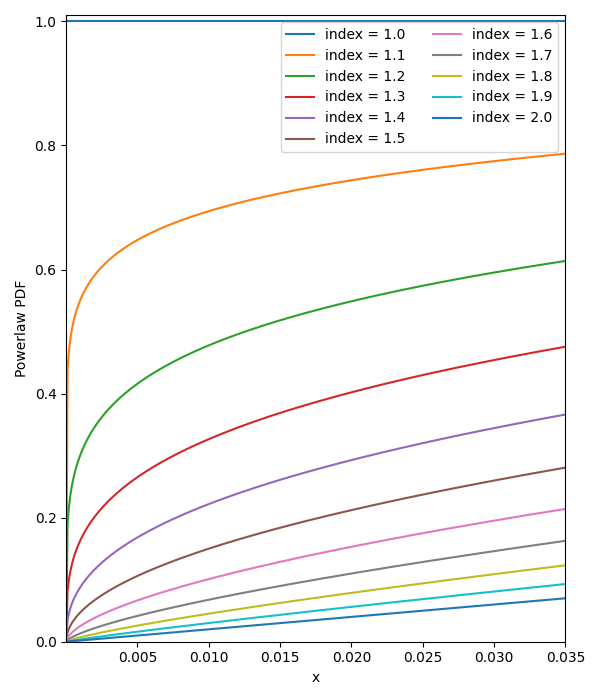
\includegraphics[width=\textwidth]{images/powerlaw}
    \captionof{figure}{Power law distribution}
\end{minipage}

\,\\\subsubsection*{\textbf{Beta distribution}}
For the beta distribution, we use the following form,
\begin{equation}
    f(x, a, b) = \frac{\Gamma(a+b)x^{a-1}(1-x)^{b-1}}{\Gamma(a)\Gamma(b)}
    \label{eq:beta_distribution}
\end{equation}
For $0 \leq x \leq 1, a > 0, b > 0$ and $\Gamma$ is the gamma function.\footnote{\url{https://docs.scipy.org/doc/scipy/reference/generated/scipy.stats.beta.html}}

Figure~\ref{fig:beta1} shows the beta distribution with a fixed $\beta=80$.
Similarly, figure~\ref{fig:beta2} shows the beta distribution with a fixed $\alpha=5$.
For our case, we selected $\text{Beta}(5, 80)$ as our distribution of choice for metallicity and generated $10^7$ values between the COMPAS limits $10^{-4} < z < 0.03$. %The same value for metallicity was used for both stars as different metallicity scenario is highly unlikely.

\begin{figure}[!ht]%
    \centering
    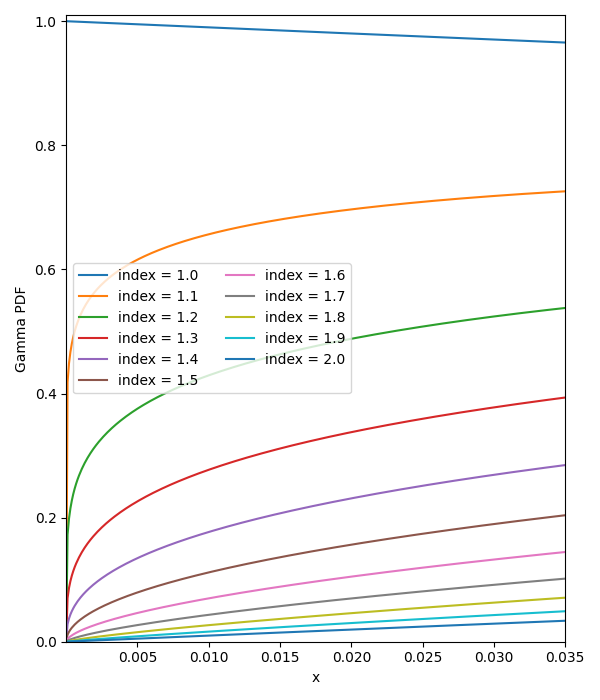
\includegraphics[width=\linewidth]{images/gamma}
    \caption{Gamma distribution with $1 \leq a \leq 2$.}
    \label{fig:gamma_distribution}
\end{figure}%
\begin{figure}[!ht]%
    \centering
    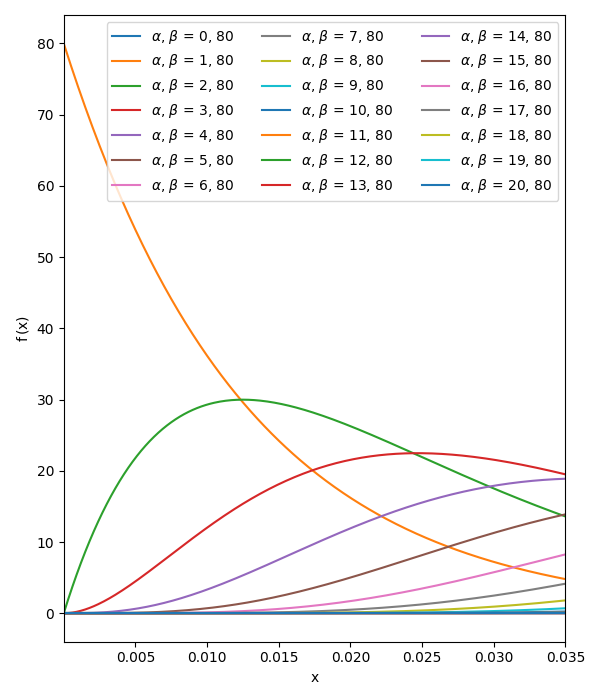
\includegraphics[width=\linewidth]{images/beta1}
    \caption{Beta distribution with varying $\alpha$ and fixed $\beta$ parameter.}
    \label{fig:beta1}
\end{figure}%
\begin{figure}[!ht]%
    \centering
    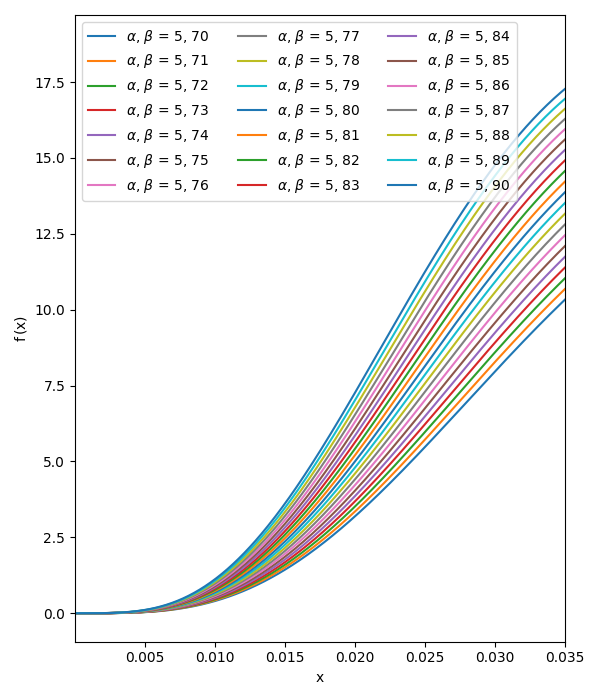
\includegraphics[width=\linewidth]{images/beta2}
    \caption{Beta distribution with fixed $\alpha$ and varying $\beta$ parameters.}
    \label{fig:beta2}
\end{figure}%

\subsection{\textbf{Metallicity}}
\label{subsec:metallicity}
One of the major challenges in generation of the stellar binaries for this study was the selection of a distribution which will result in stars at the higher end of COMPAS metallicity boundary, $z = 0.03$.
A power-law, gamma, and beta distributions were selected to try and simulate the required metallicity distribution.
In the following section, we discuss the selected distributions briefly,
    \newpage
    \section{Milky way Model}
\label{sec:milky_way}
In this section, we will briefly outline the milky way galaxy model used in this study.
The model is developed by~\cite{wagg2021gravitational} and makes use of the galaxy's enrichment history by taking
into account the metallicity-radius-time relationship~\cite{Frankel2018}.
It uses a separate star formation history and spatial distribution for the \lowalpha, \highalpha\ discs, and bulge in the galaxy.

\subsection{Star formation rate}
\label{subsec:star_formation_rate}
The star formation rate for both the \lowalpha\ and \highalpha\ disks is expressed as,
\begin{equation}
    p(\tau) \propto \exp\left(-\frac{\tau_m - \tau}{\tau_\text{SFR}}\right),
    \label{eq:star_formation_rate_equation}
\end{equation}
where $\tau$ is the time difference between the star's ZAMS stage and today.
The age of milky way galaxy, $\tau_m$, is taken as \SI{12}{\giga\yr}, and the star formation rate as, $\tau_\text{
    SFR}\ $= \SI{6.8}{\giga\yr}.
The star-forming period of \lowalpha\ and \highalpha\ discs were taken as \SIrange{0}{8}{\giga\yr} and \SIrange{8}{12}{\giga\yr} respectively.
The model adopts \SIrange{6}{12}{\giga\yr} as the star-forming period of the bulge~\cite{Bovy2019}.

\subsection{Radial distribution}
\label{subsec:radial_distribution}
The radial distribution of stars within the milky way galaxy was performed using the following expression,
\begin{equation}%
    p(R) = \exp\left(-\frac{R}{R_d}\right)\frac{R}{R_d^2}
    \label{eq:radial_distribution_of_stars}
\end{equation}%

However, a different scale length, $R_d$, was chosen for each component of the galaxy.
For \lowalpha, the model uses $R_\text{exp}(\tau)$ as the scale length~\cite[Eq 6]{Frankel2018}, where

\begin{equation}%
    R_\text{exp}(\tau) = 4\,\text{kpc}\left[1 - \alpha_{R_\text{exp}}\left(\frac{\tau}{8\,\text{Gyr}}\right)\right],
    \label{eq:exponential_radius_equation}
\end{equation}%
with the value of inside-out growth parameter, $\alpha_{R_\text{exp}}$, as 0.3. For \highalpha\ disc and bulge, the value of scale length was chosen as $(1/0.43)\,$\si{\kpc} and \SI{1.5}{\kpc} respectively.

\subsection{Vertical distribution}
\label{subsec:vertical_distribution}
The model employs a similar method of single exponent expression with varying scale height parameters for the vertical distribution as well.
The exponential expression used is,
\begin{equation}
    p(|z|) = \frac{1}{z_d}\exp\left(-\frac{z}{z_d}\right),
    \label{eq:vertical_distribution_of_stars}
\end{equation}
where $z$ here is the vertical displacement from the galactic plane.
The scale height parameter, $z_d$, for \lowalpha, \highalpha\ and bulge was taken as \SI{0.3}{\kpc}~\cite{McMillan2011}, \SI{0.95}{\kpc}~\cite{Bovy2016}, and \SI{0.2}{\kpc}~\cite{Wegg2015} respectively.

\subsection{Metallicity-radius-time relationship}
\label{subsec:metallicity_radius_relationship}
The MRT relationship plays an important part, both in the galaxy model and later on in the placement of DCOs within the galaxy as well.
The model makes use of~\cite[Eq. 7]{Frankel2018},
\begin{equation}
    \feh(R,\tau) = F_m + \nabla\feh R - \left(F_m + \nabla\feh R_{\feh=0}^{\text{now}}\right) f(\tau)
\end{equation}
For each point generated, if the value of metallicity produced by the MW model was less or greater than the limits defined by COMPAS\footnote{0.0001, 0.03} it was changed to a uniformly drawn random number between $\text{COMPAS}_\text{min} - \text{ZSOLAR}$ and $\text{ZSOLAR} - \text{COMPAS}_\text{max}$ respectively.
\subsection{Galaxy synthesis}
\label{subsec:galaxy_synthesis}
For the synthesis of an instance of the Milky Way galaxy, the model described previously samples the following parameters,
\begin{equation*}
    \theta_i = \{\tau, D, z, \text{component}\},
\end{equation*}
where $\tau$ is the look-back time for the binary, $D$ is the distance from Earth, $z$ is the metallicity, and `component' is the component of the galaxy in which the binary resides.\footnote{One of the three, \lowalpha\ disc, \highalpha\ disc, or bulge.}
The parameters are generated for $i = 1, 2, 3, \ldots$, $N_\text{GAL}$, where $N_\text{GAL} = 100$.
    \newpage
    \section{Parameter distribution across the galaxies}
\label{sec:paramter-distribution-across-the-galaxies}
\subsection{Binary Black Holes}
\begin{figure}[!h]
    \centering
    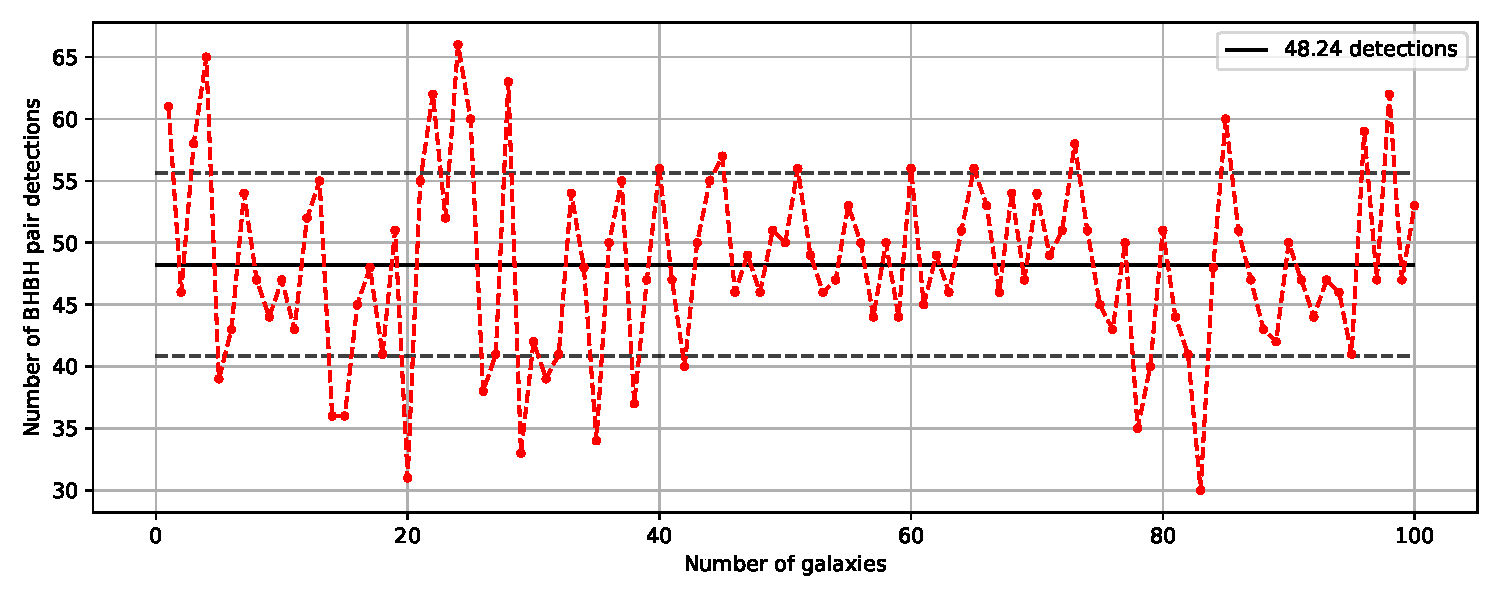
\includegraphics[width=\columnwidth]{analysis_data/main_analysis_folder/BHBH_n_detections}
    \caption{Number of BHBH pair detection per galaxy instance. On average, a total of $\sim$48 pairs per galaxy were detected in this study.}
    \label{fig:bhbhndetections}
\end{figure}

\begin{figure}[!h]
    \centering
    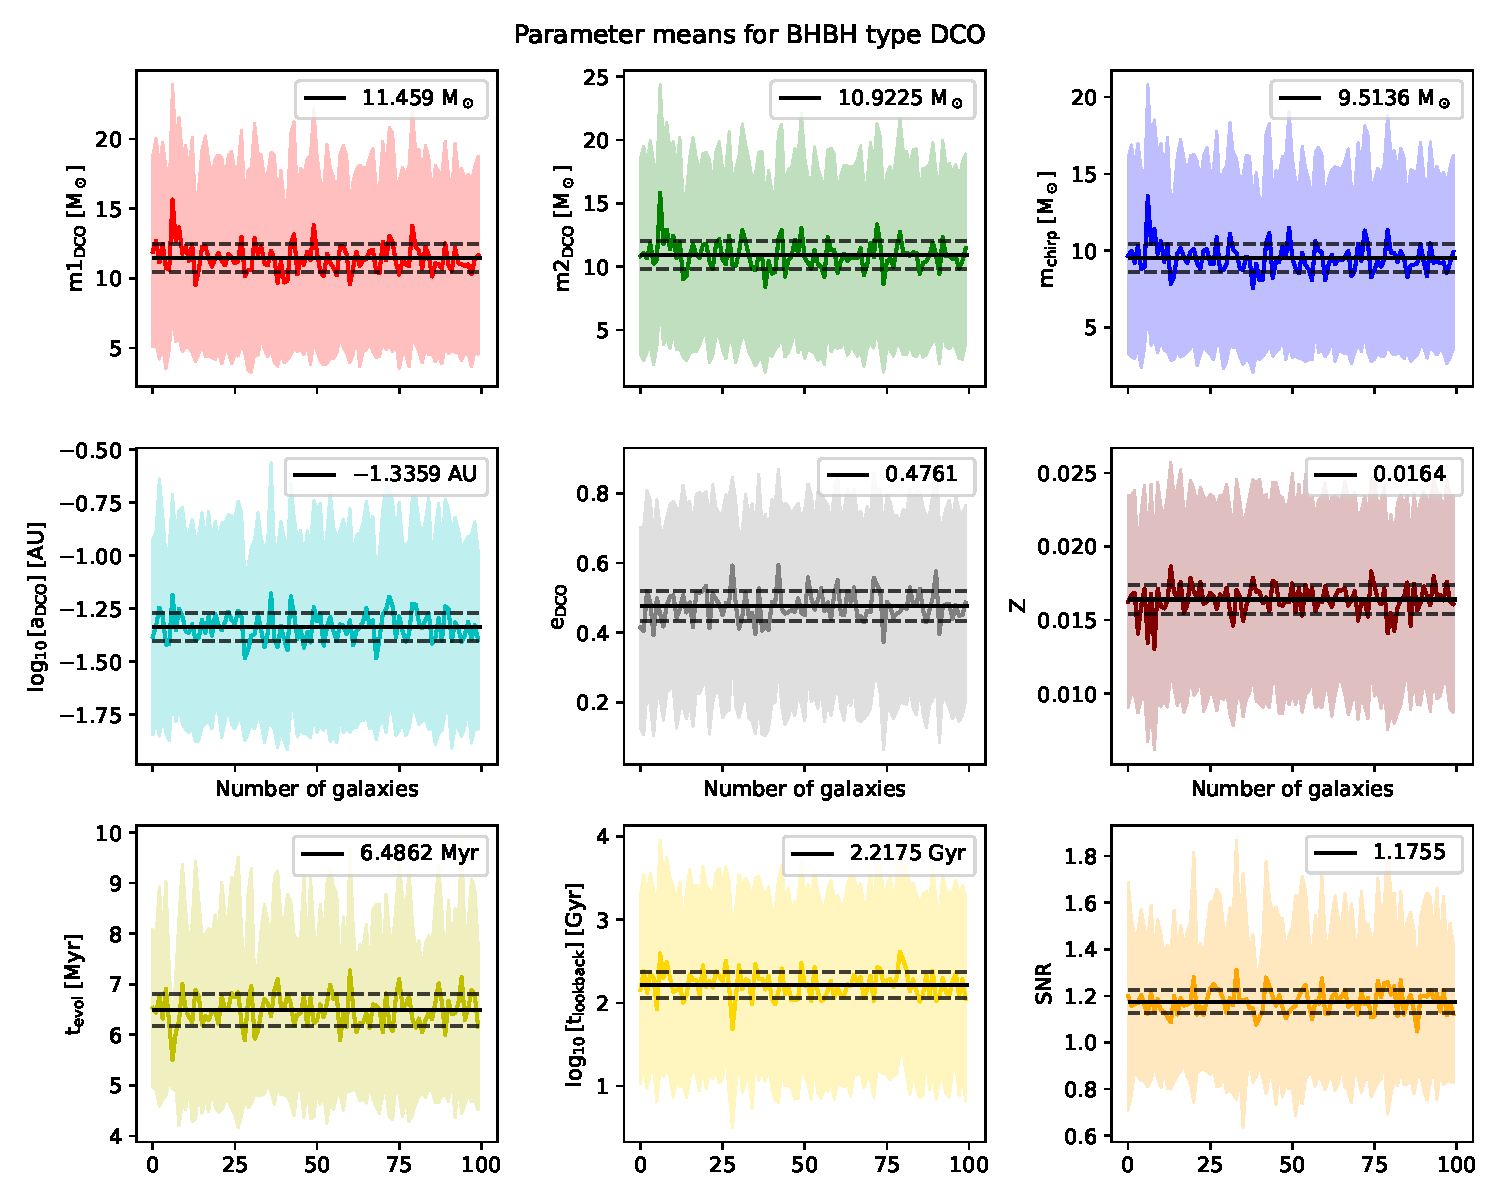
\includegraphics[width=\columnwidth]{analysis_data/main_analysis_folder/BHBH_n_galaxy_mean_plot}
    \caption{The mean and standard deviation for selected parameters in every galaxy is plotted against the galaxy number. An overall measure of mean and standard deviation of all the galaxies is also shown for selected parameter with a black solid and dashed lines respectively.}
    \label{fig:bhbh_n_galaxy_mean_plot}
\end{figure}

\subsection{Binary Neutron Stars}
\begin{figure}[!h]
	\centering
	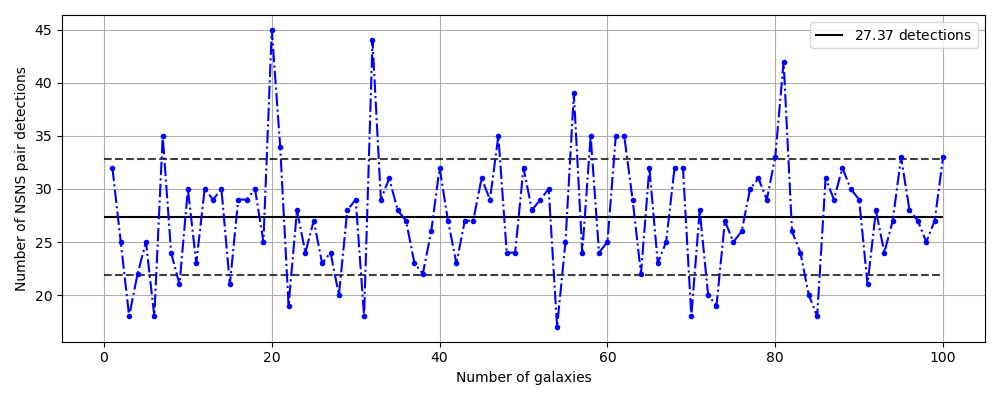
\includegraphics[width=\columnwidth]{analysis_data/main_analysis_folder/NSNS_n_detections}
	\caption{Number of NSNS pair detection per galaxy instance. On average, a total of $\sim$27 pairs per galaxy were detected in this study.}
	\label{fig:nsnsndetections}
\end{figure}

\begin{figure}[!h]
	\centering
	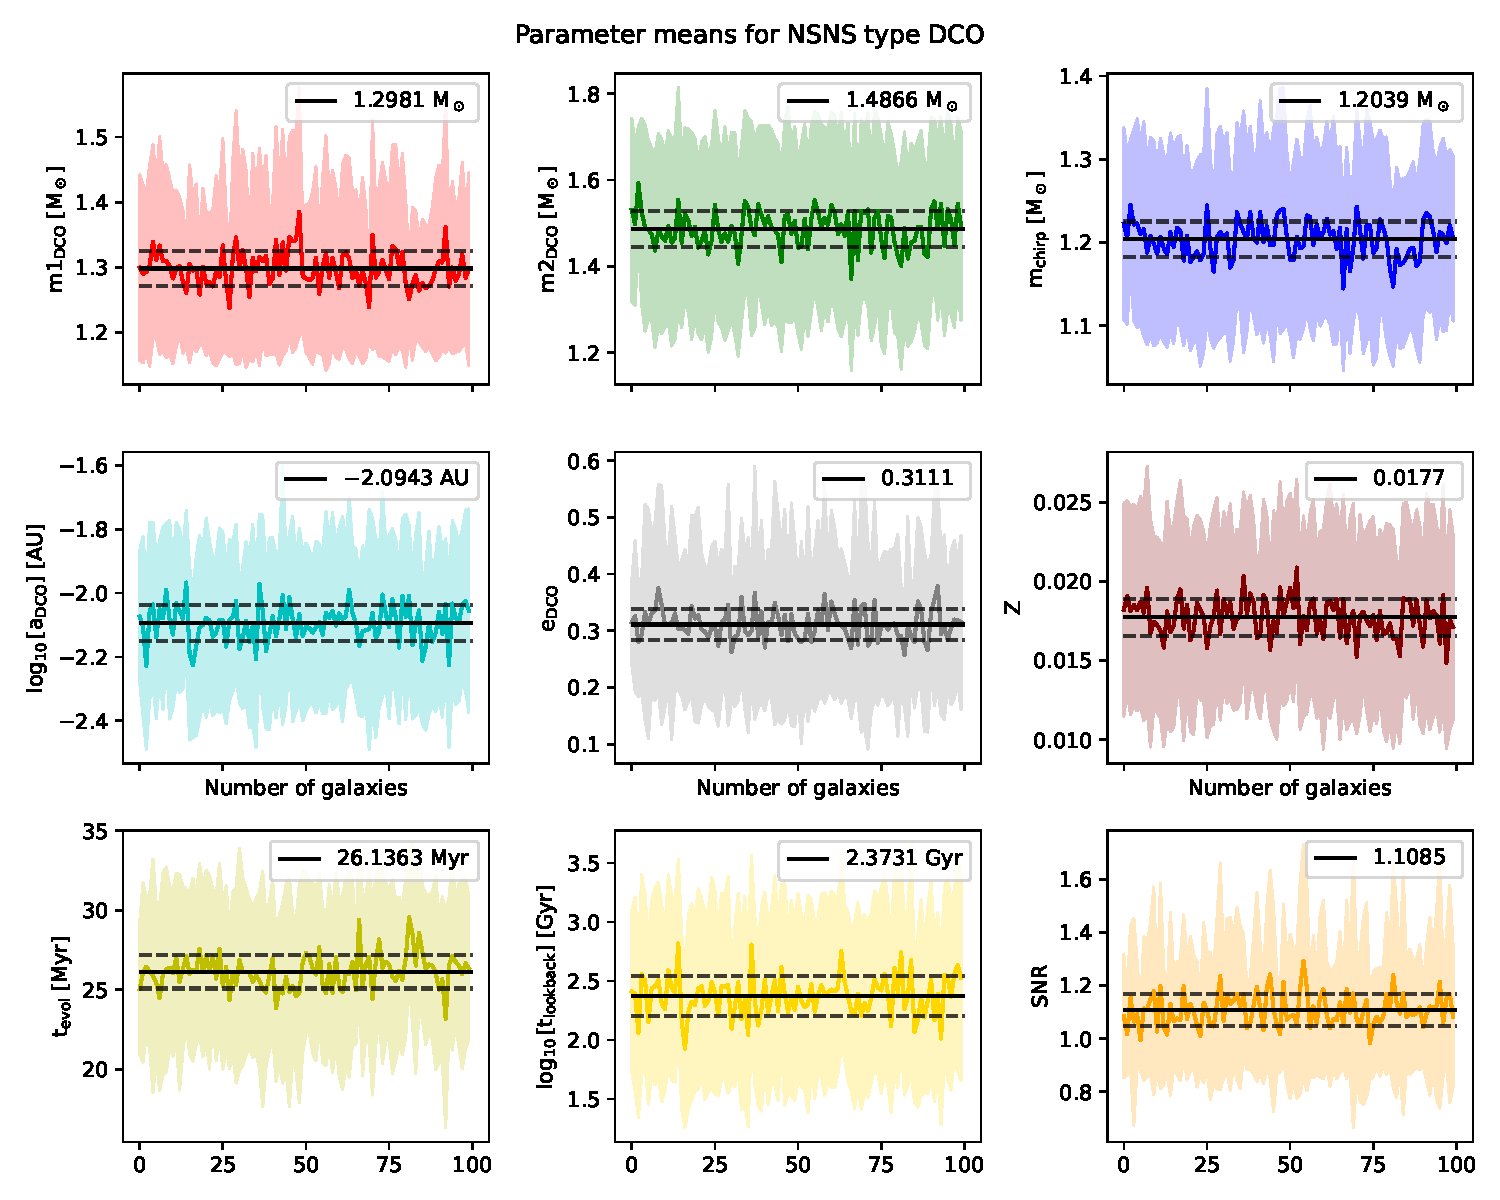
\includegraphics[width=\columnwidth]{analysis_data/main_analysis_folder/NSNS_n_galaxy_mean_plot}
	\caption{Same as figure~\ref{fig:bhbh_n_galaxy_mean_plot}.}
	\label{fig:nsns_n_galaxy_mean_plot}
\end{figure}

\subsection{Neutron Star $-$ Black Hole binary}

\begin{figure}[!h]
	\centering
	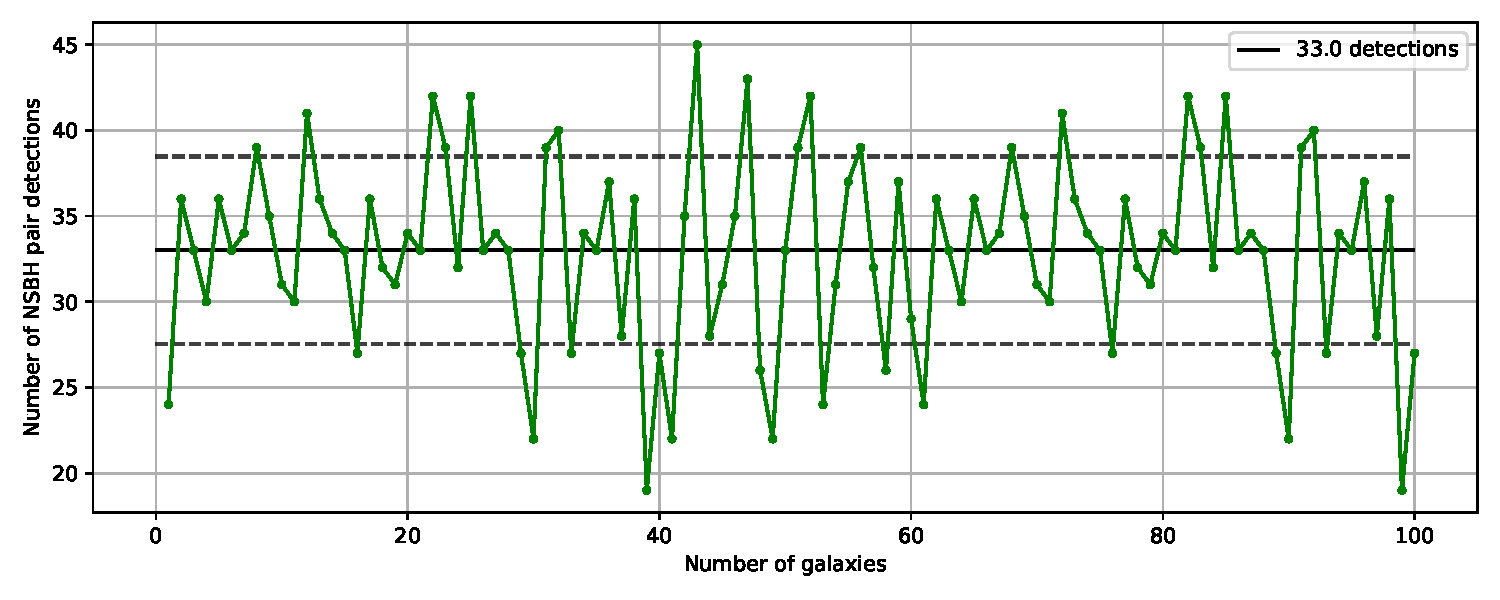
\includegraphics[width=\columnwidth]{analysis_data/main_analysis_folder/NSBH_n_detections}
	\caption{Number of NSBH pair detection per galaxy instance. On average, a total of $\sim$32 pairs per galaxy were detected in this study.}
	\label{fig:nsbhndetections}
\end{figure}	

\begin{figure}[!h]
	\centering
	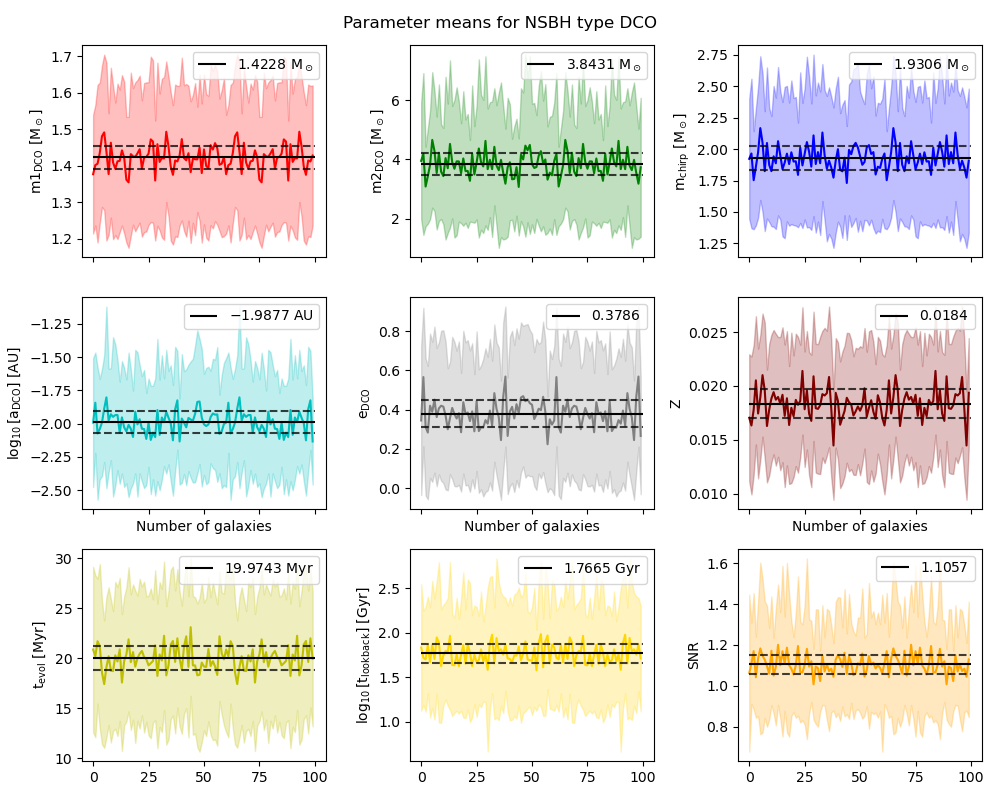
\includegraphics[width=\columnwidth]{analysis_data/main_analysis_folder/NSBH_n_galaxy_mean_plot}
	\caption{Same as figure~\ref{fig:bhbh_n_galaxy_mean_plot}.}
	\label{fig:nsbh_n_galaxy_mean_plot}
\end{figure}

\newpage
\subsection{Black Hole $-$ Neutron Star binary}
\begin{figure}[!h]
	\centering
	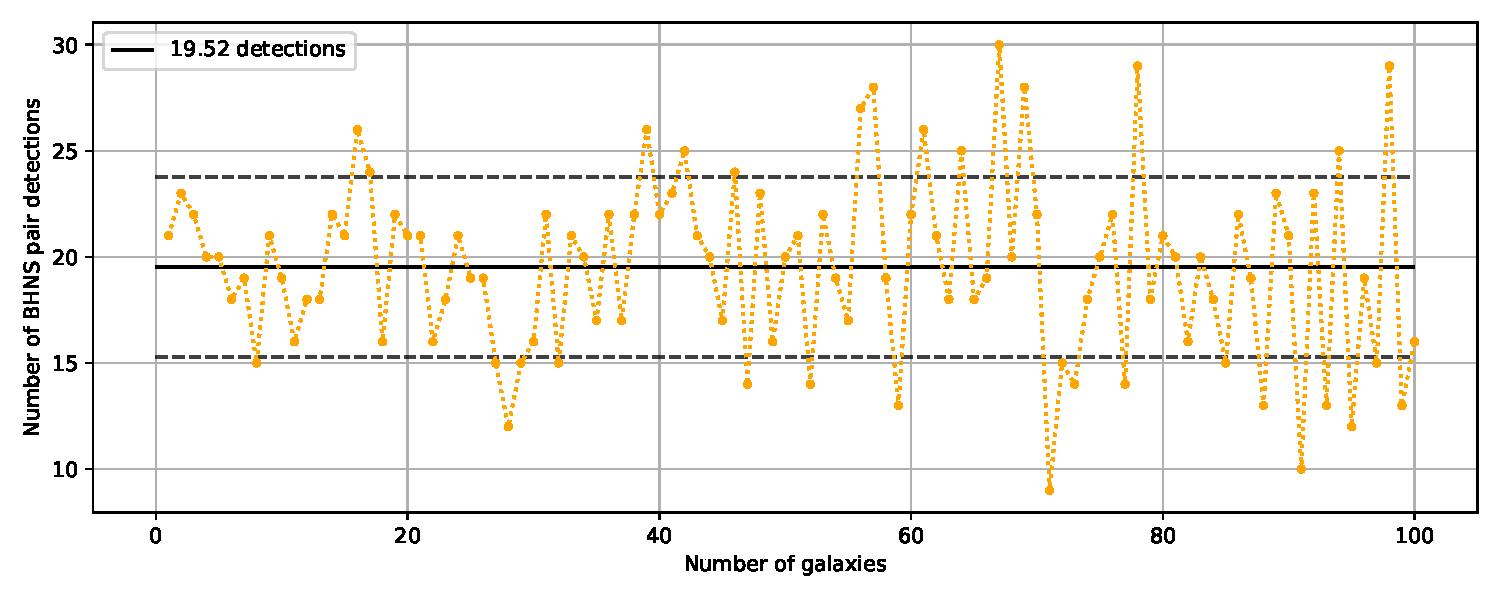
\includegraphics[width=\columnwidth]{analysis_data/main_analysis_folder/BHNS_n_detections}
	\caption{Number of BHNS pair detection per galaxy instance. On average, a total of $\sim$19 pairs per galaxy were detected in this study.}
	\label{fig:bhnsndetections}
\end{figure}	

\begin{figure}[!h]
	\centering
	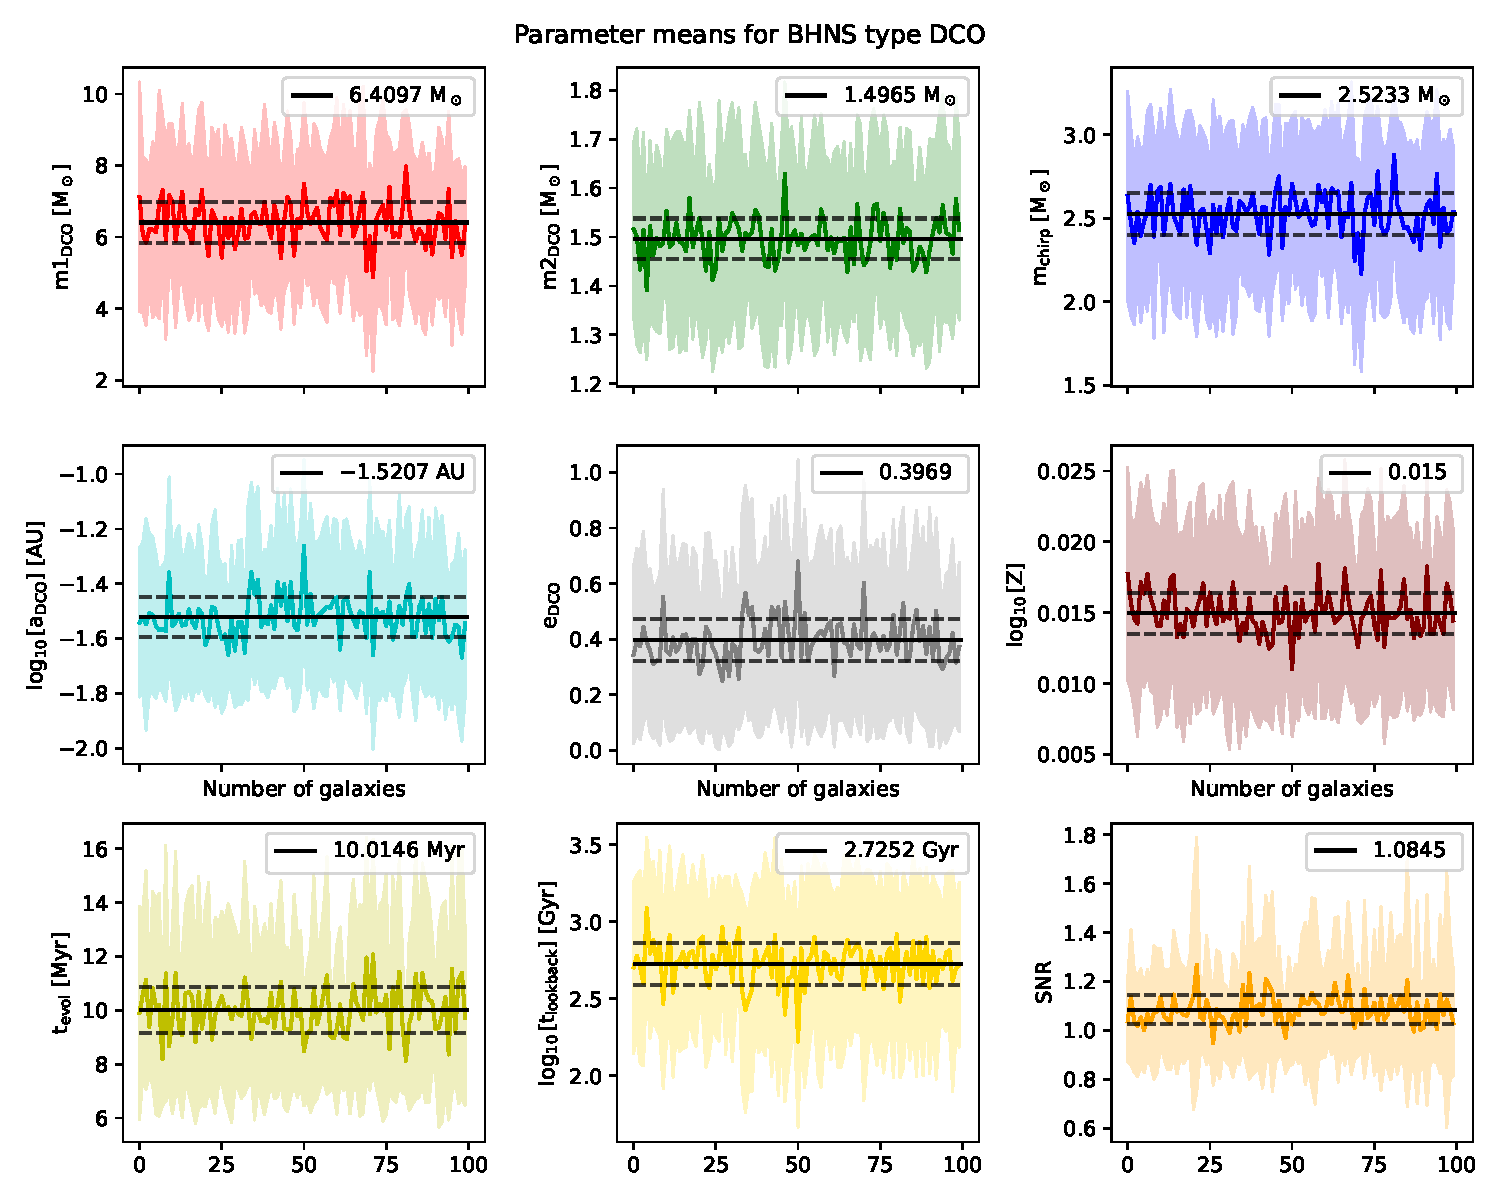
\includegraphics[width=\columnwidth]{analysis_data/main_analysis_folder/BHNS_n_galaxy_mean_plot}
	\caption{Same as figure~\ref{fig:bhbh_n_galaxy_mean_plot}.}
	\label{fig:bhns_n_galaxy_mean_plot}
\end{figure}

    \newpage
    \section{Parameter distribution across the galaxies $-\ \Theta_2$}
\label{sec:paramter-distribution-across-the-galaxies-theta-2}

\subsection{Binary Black Holes}
\begin{figure}[!h]
    \centering
    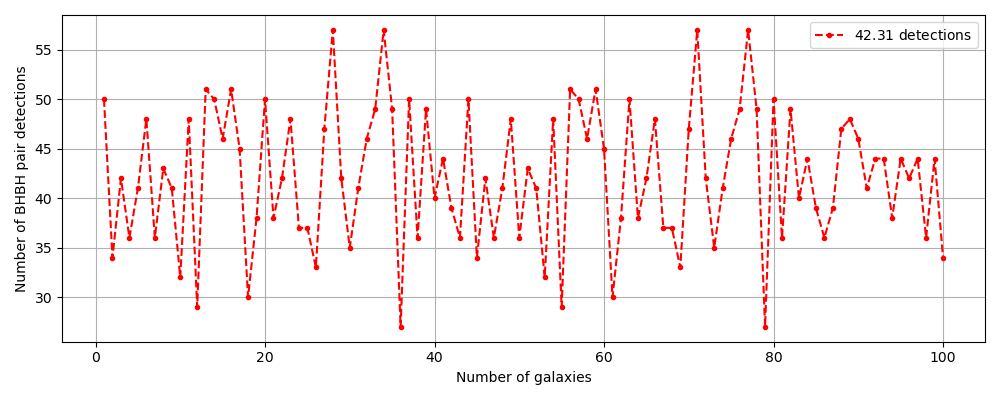
\includegraphics[width=\columnwidth]{analysis_data/004__images_for_latex/BHBH0e_n_detections}
    \caption{Number of BHBH pair detection per galaxy instance. On average, a total of $\sim$42 pairs per galaxy were detected in this study.}
    \label{fig:bhbh0endetections}
\end{figure}

\begin{figure}[!h]
    \centering
    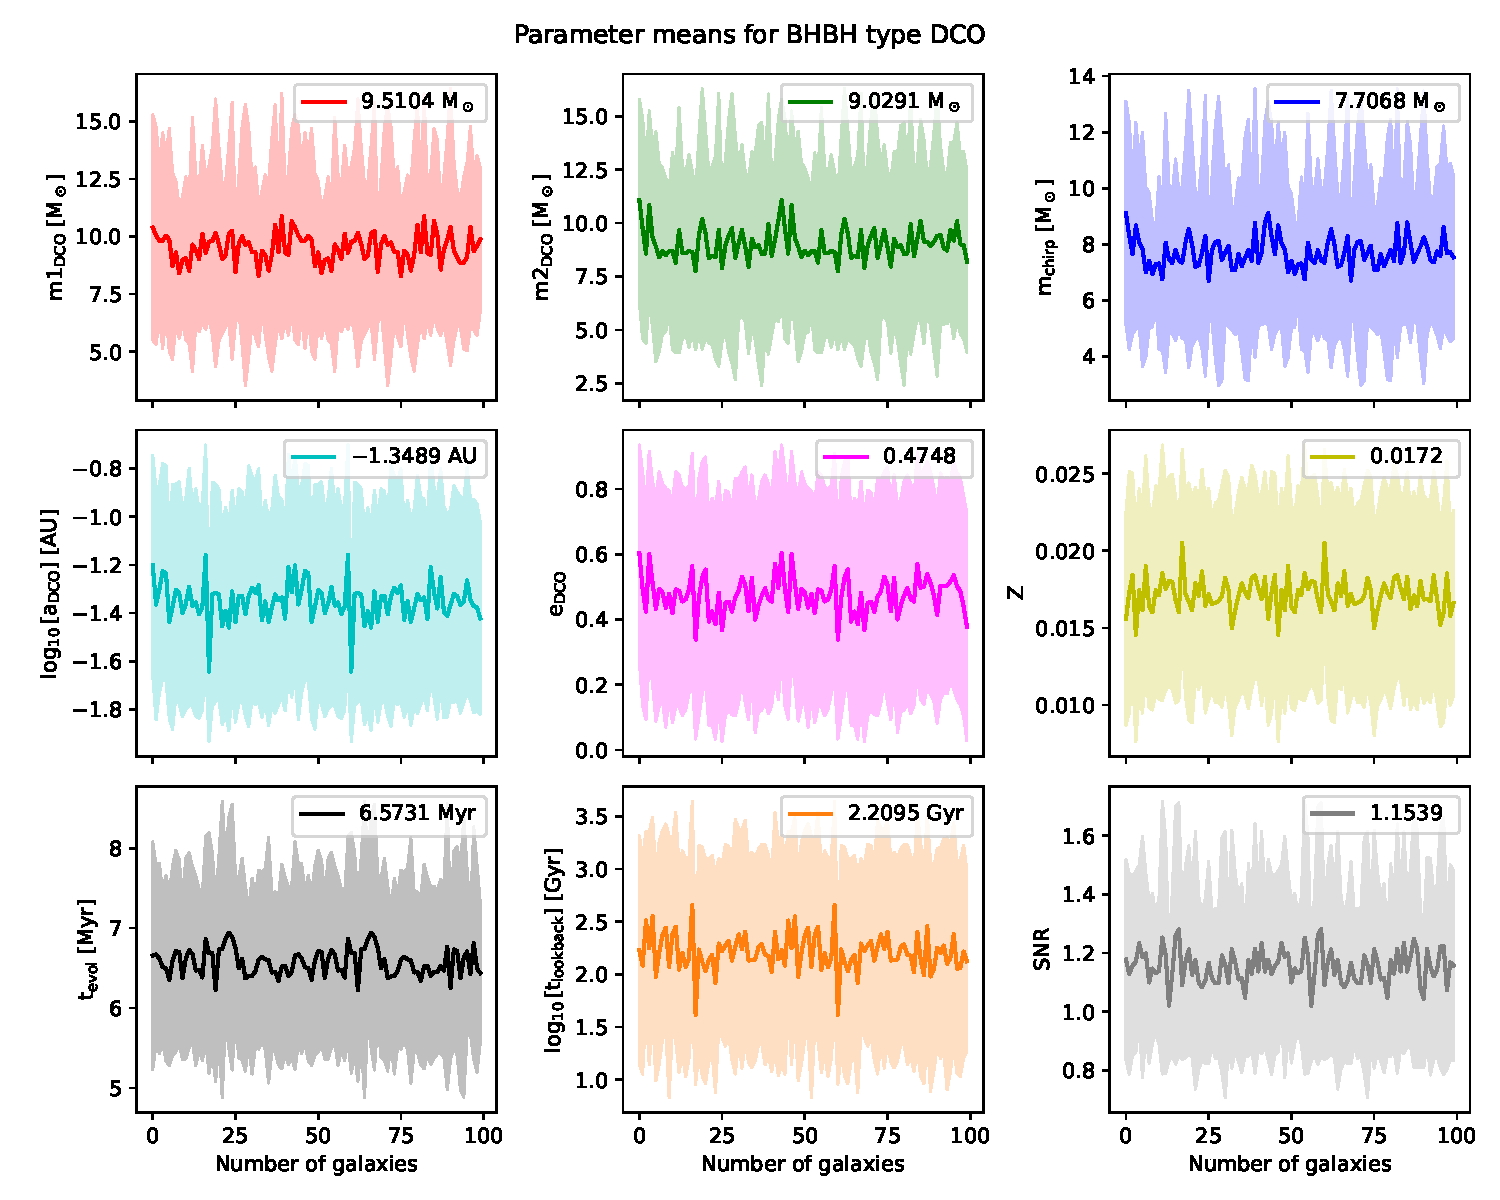
\includegraphics[width=\columnwidth]{analysis_data/004__images_for_latex/BHBH0e_n_galaxy_mean_plot}
    \caption{The mean and standard deviation for selected parameters in every galaxy, plotted against the galaxy number. An overall measure of mean and standard deviation of all the galaxies is also shown for the selected parameters.}
    \label{fig:bhbh0e_n_galaxy_mean_plot}
\end{figure}

\subsection{Binary Neutron Stars}
\begin{figure}[!h]
    \centering
    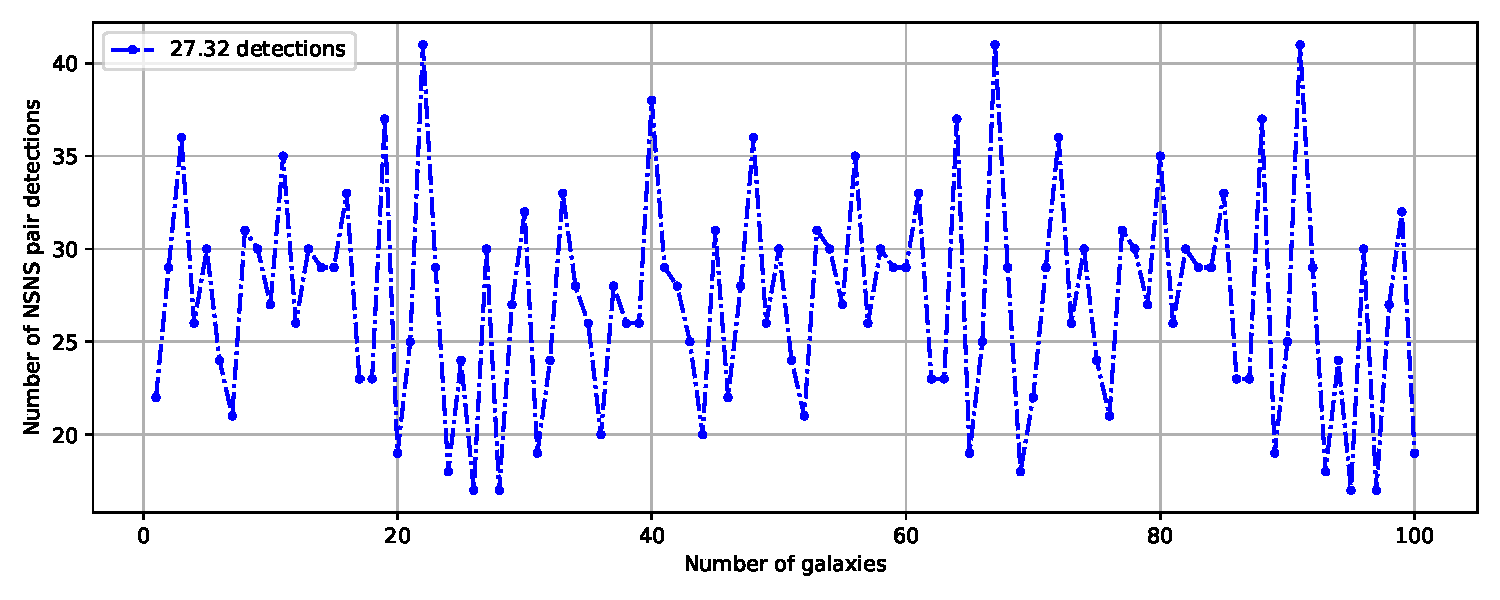
\includegraphics[width=\columnwidth]{analysis_data/004__images_for_latex/NSNS0e_n_detections}
    \caption{Number of NSNS pair detection per galaxy instance. On average, a total of $\sim$27 pairs per galaxy were detected in this study.}
    \label{fig:nsns0endetections}
\end{figure}

\begin{figure}[!h]
    \centering
    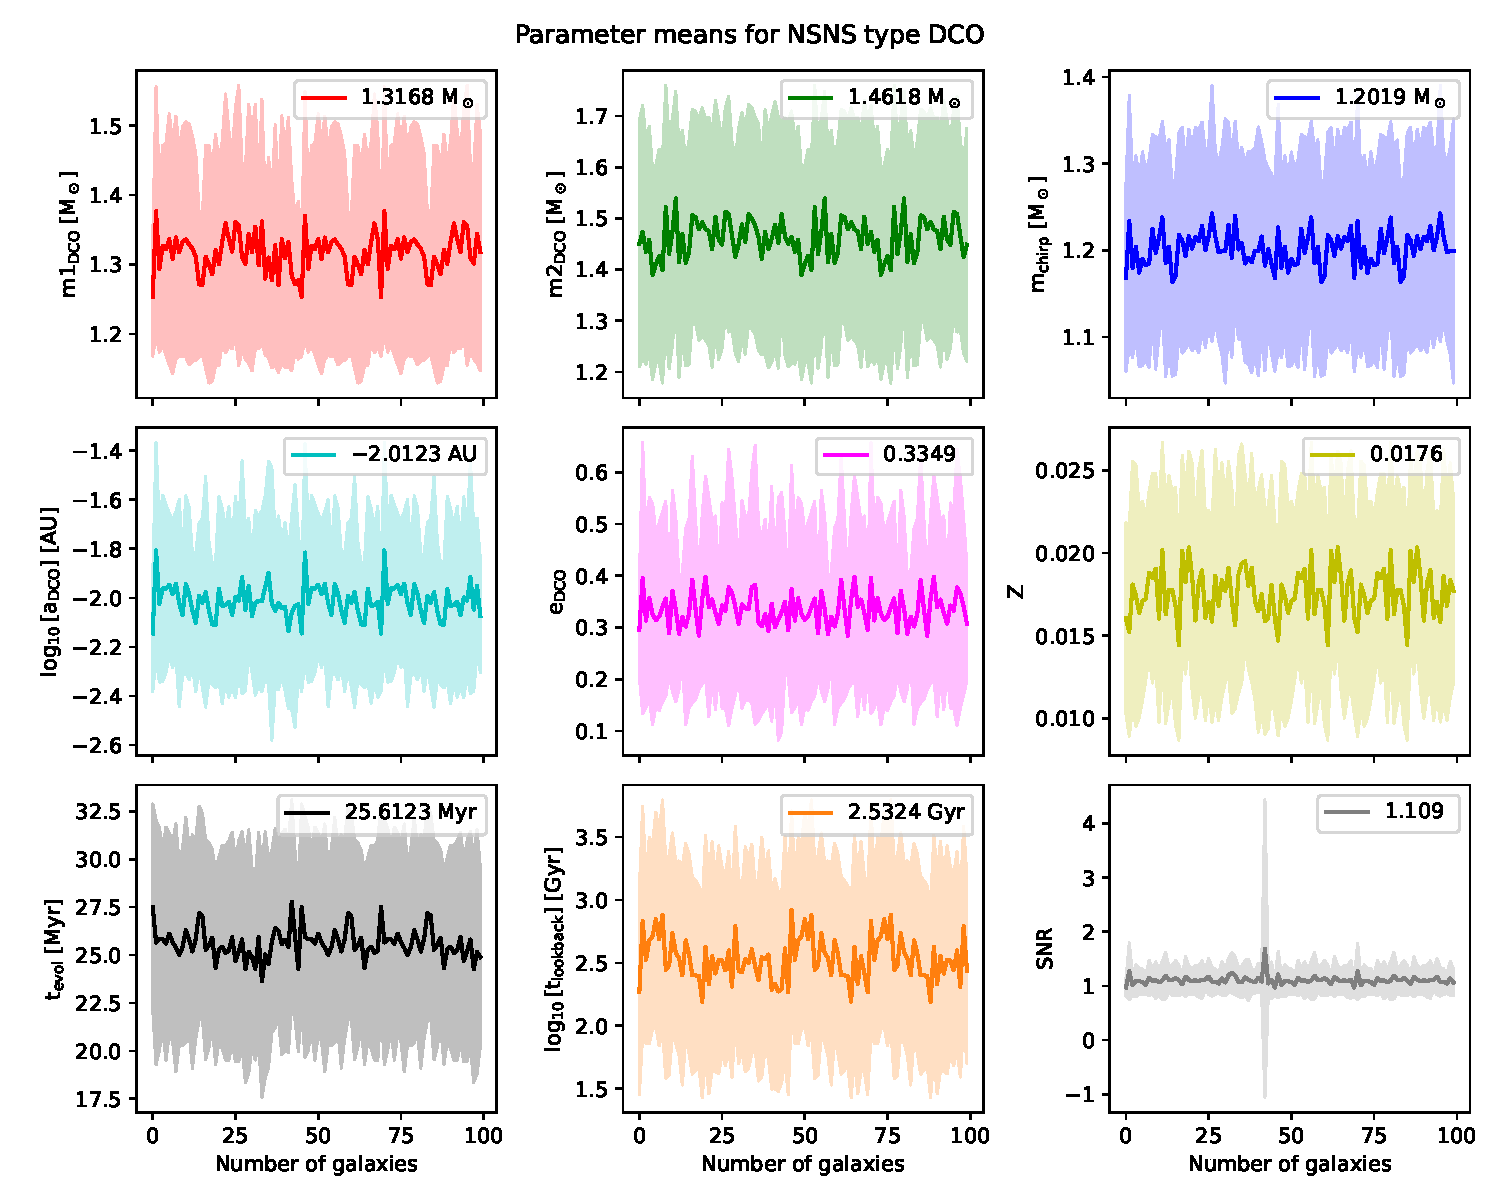
\includegraphics[width=\columnwidth]{analysis_data/004__images_for_latex/NSNS0e_n_galaxy_mean_plot}
    \caption{Same as figure~\ref{fig:bhbh0e_n_galaxy_mean_plot}.}
    \label{fig:nsns0e_n_galaxy_mean_plot}
\end{figure}

\subsection{Black Hole $-$ Neutron Star binary}
\begin{figure}[!h]
    \centering
    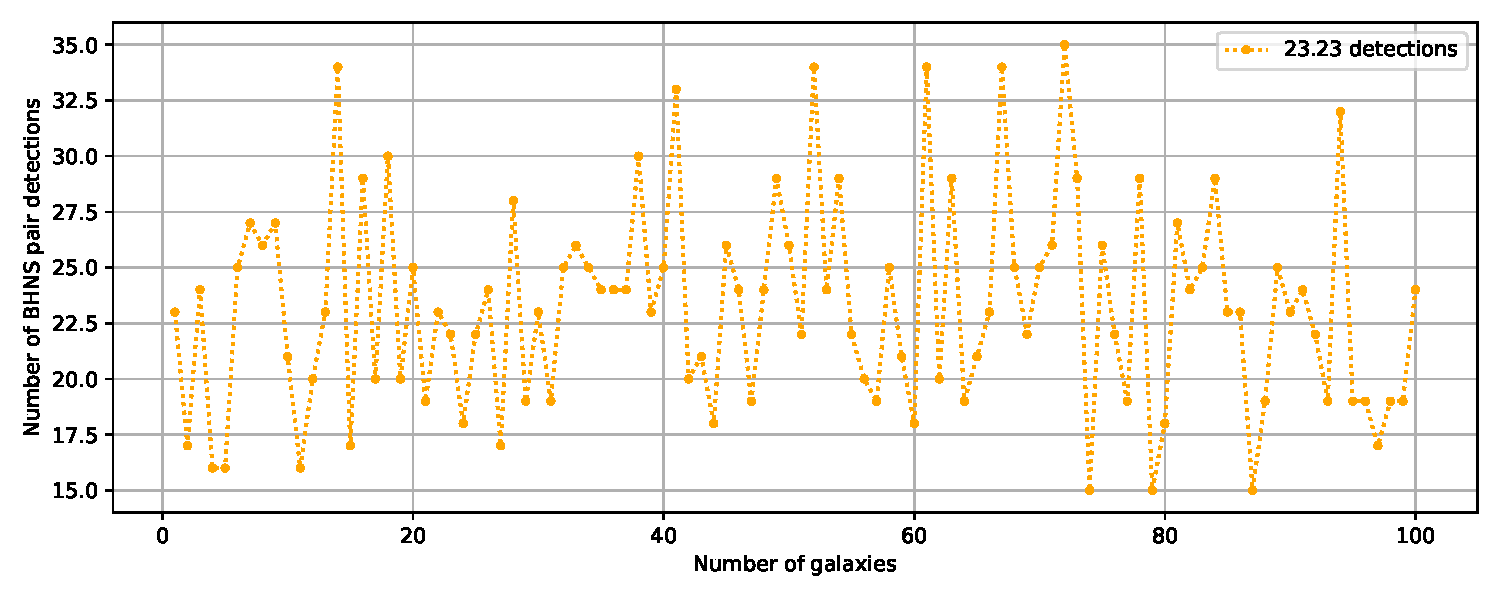
\includegraphics[width=\columnwidth]{analysis_data/004__images_for_latex/BHNS0e_n_detections}
    \caption{Number of BHNS pair detection per galaxy instance. On average, a total of $\sim$23 pairs per galaxy were detected in this study.}
    \label{fig:bhns0endetections}
\end{figure}

\begin{figure}[!h]
    \centering
    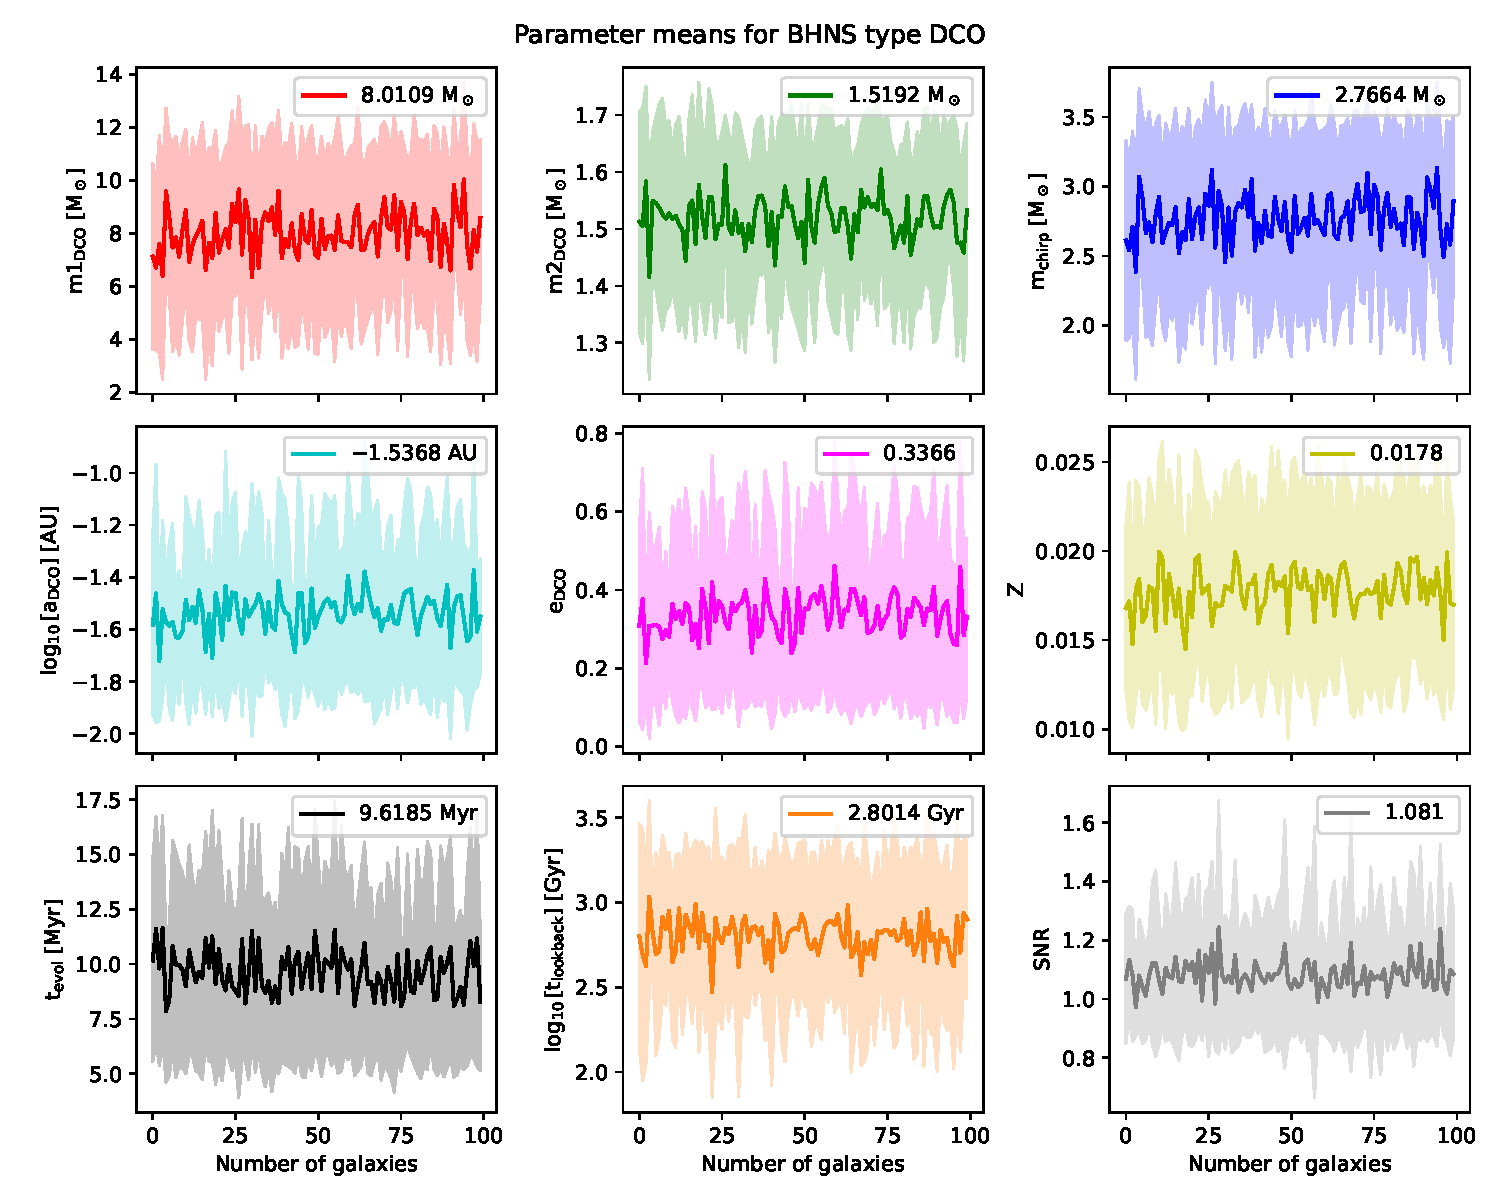
\includegraphics[width=\columnwidth]{analysis_data/004__images_for_latex/BHNS0e_n_galaxy_mean_plot}
    \caption{Same as figure~\ref{fig:bhbh0e_n_galaxy_mean_plot}.}
    \label{fig:bhns0e_n_galaxy_mean_plot}
\end{figure}

\subsection{Neutron Star $-$ Black Hole binary}
\begin{figure}[!h]
	\centering
	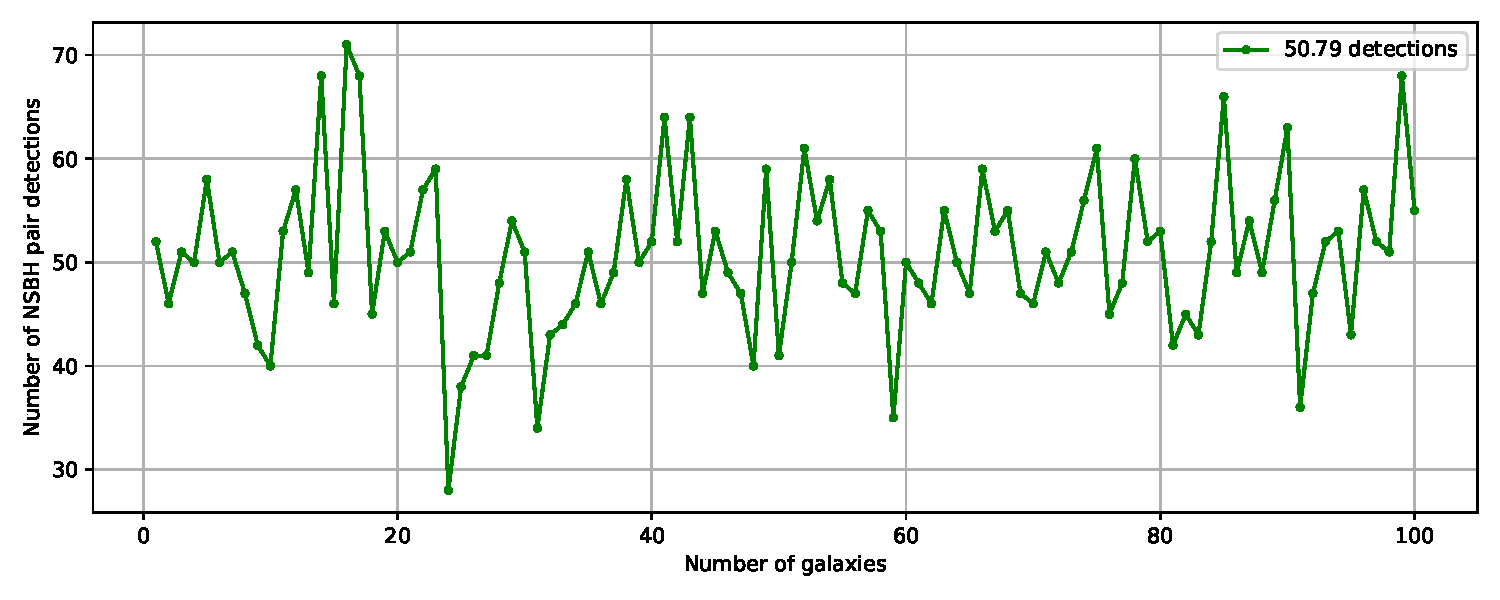
\includegraphics[width=\columnwidth]{analysis_data/004__images_for_latex/NSBH0e_n_detections}
	\caption{Number of NSBH pair detection per galaxy instance. On average, a total of $\sim$51 pairs per galaxy were detected in this study.}
	\label{fig:nsbh0endetections}
\end{figure}

\begin{figure}[!h]
	\centering
	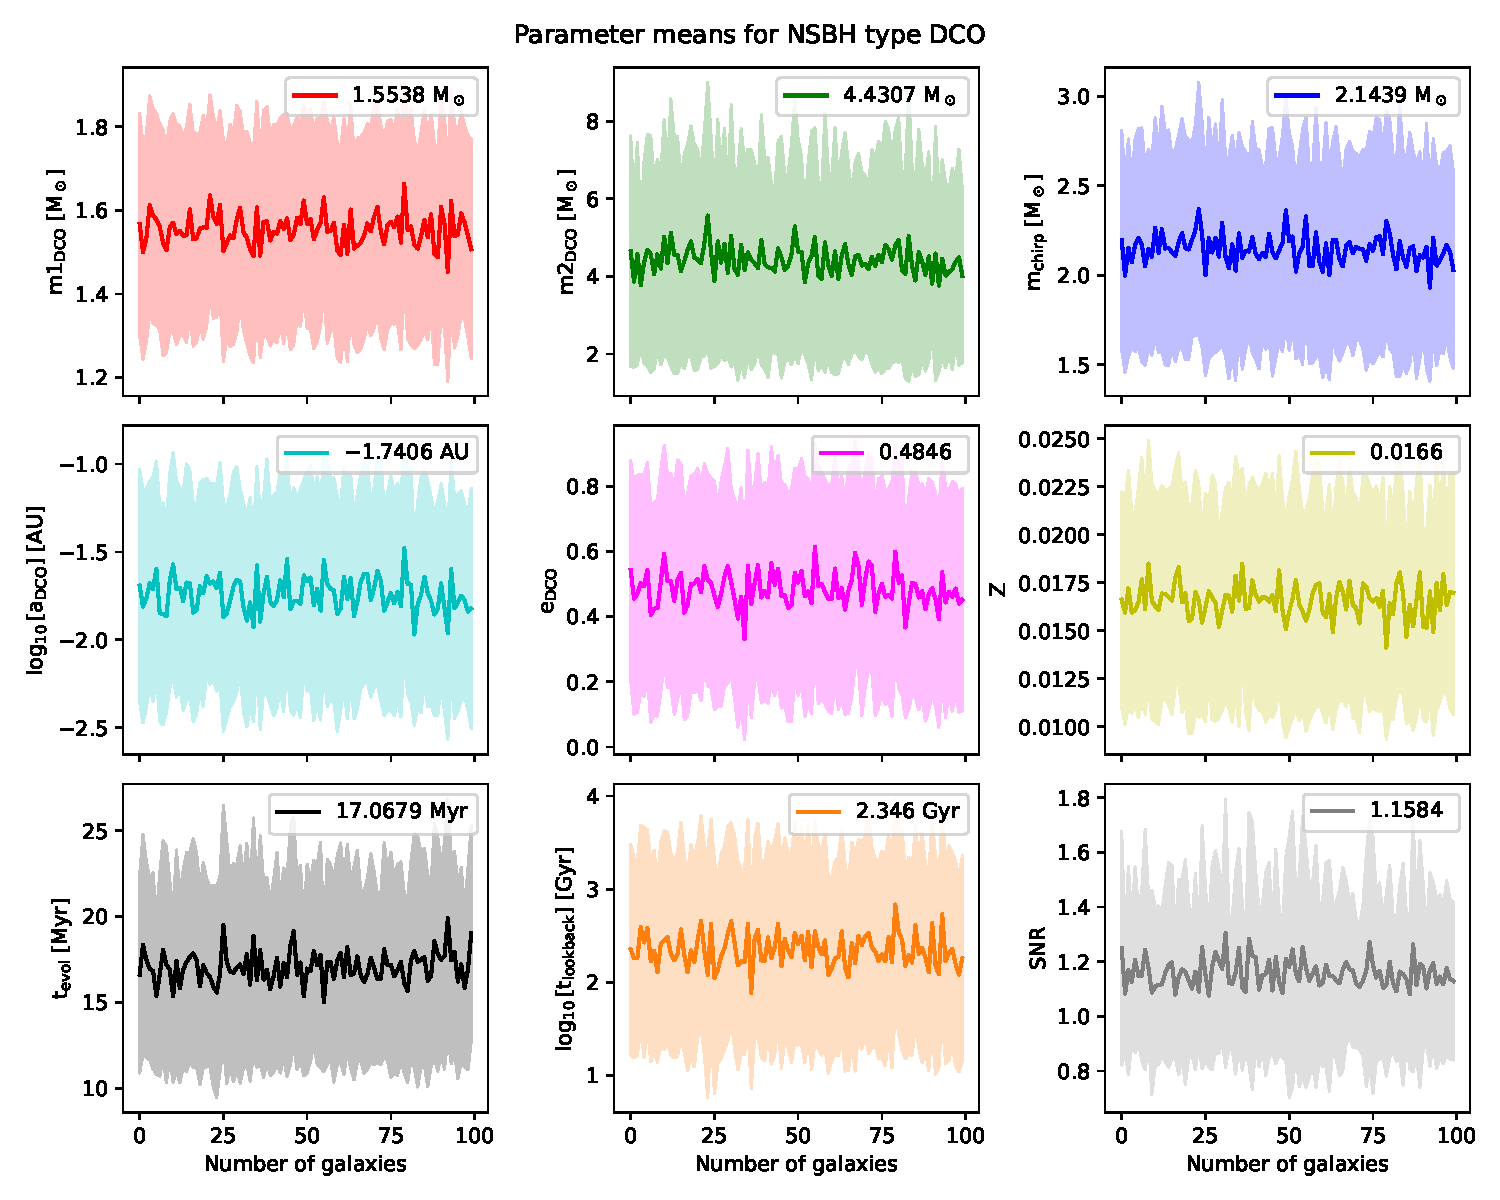
\includegraphics[width=\columnwidth]{analysis_data/004__images_for_latex/NSBH0e_n_galaxy_mean_plot}
	\caption{Same as figure~\ref{fig:bhbh0e_n_galaxy_mean_plot}.}
	\label{fig:nsbh0e_n_galaxy_mean_plot}
\end{figure}


\end{document}
